\chapter{Modèle SIR} \label{ch:SIR}

\section{Mesures et méthodologie SIR}

Les mesures ainsi que la méthodologie est la même que pour le modèle SI, c'est-à-dire que les densité $\frac{1}{2},\frac{1}{4},\frac{1}{8},\frac{1}{16}$ et les tailles de populations $5000,20000,50000,100000$ sont étudiées.

\newpage

\section{Résultats}

\begin{figure}[h]
	\centering
	\captionsetup{justification=centering}
	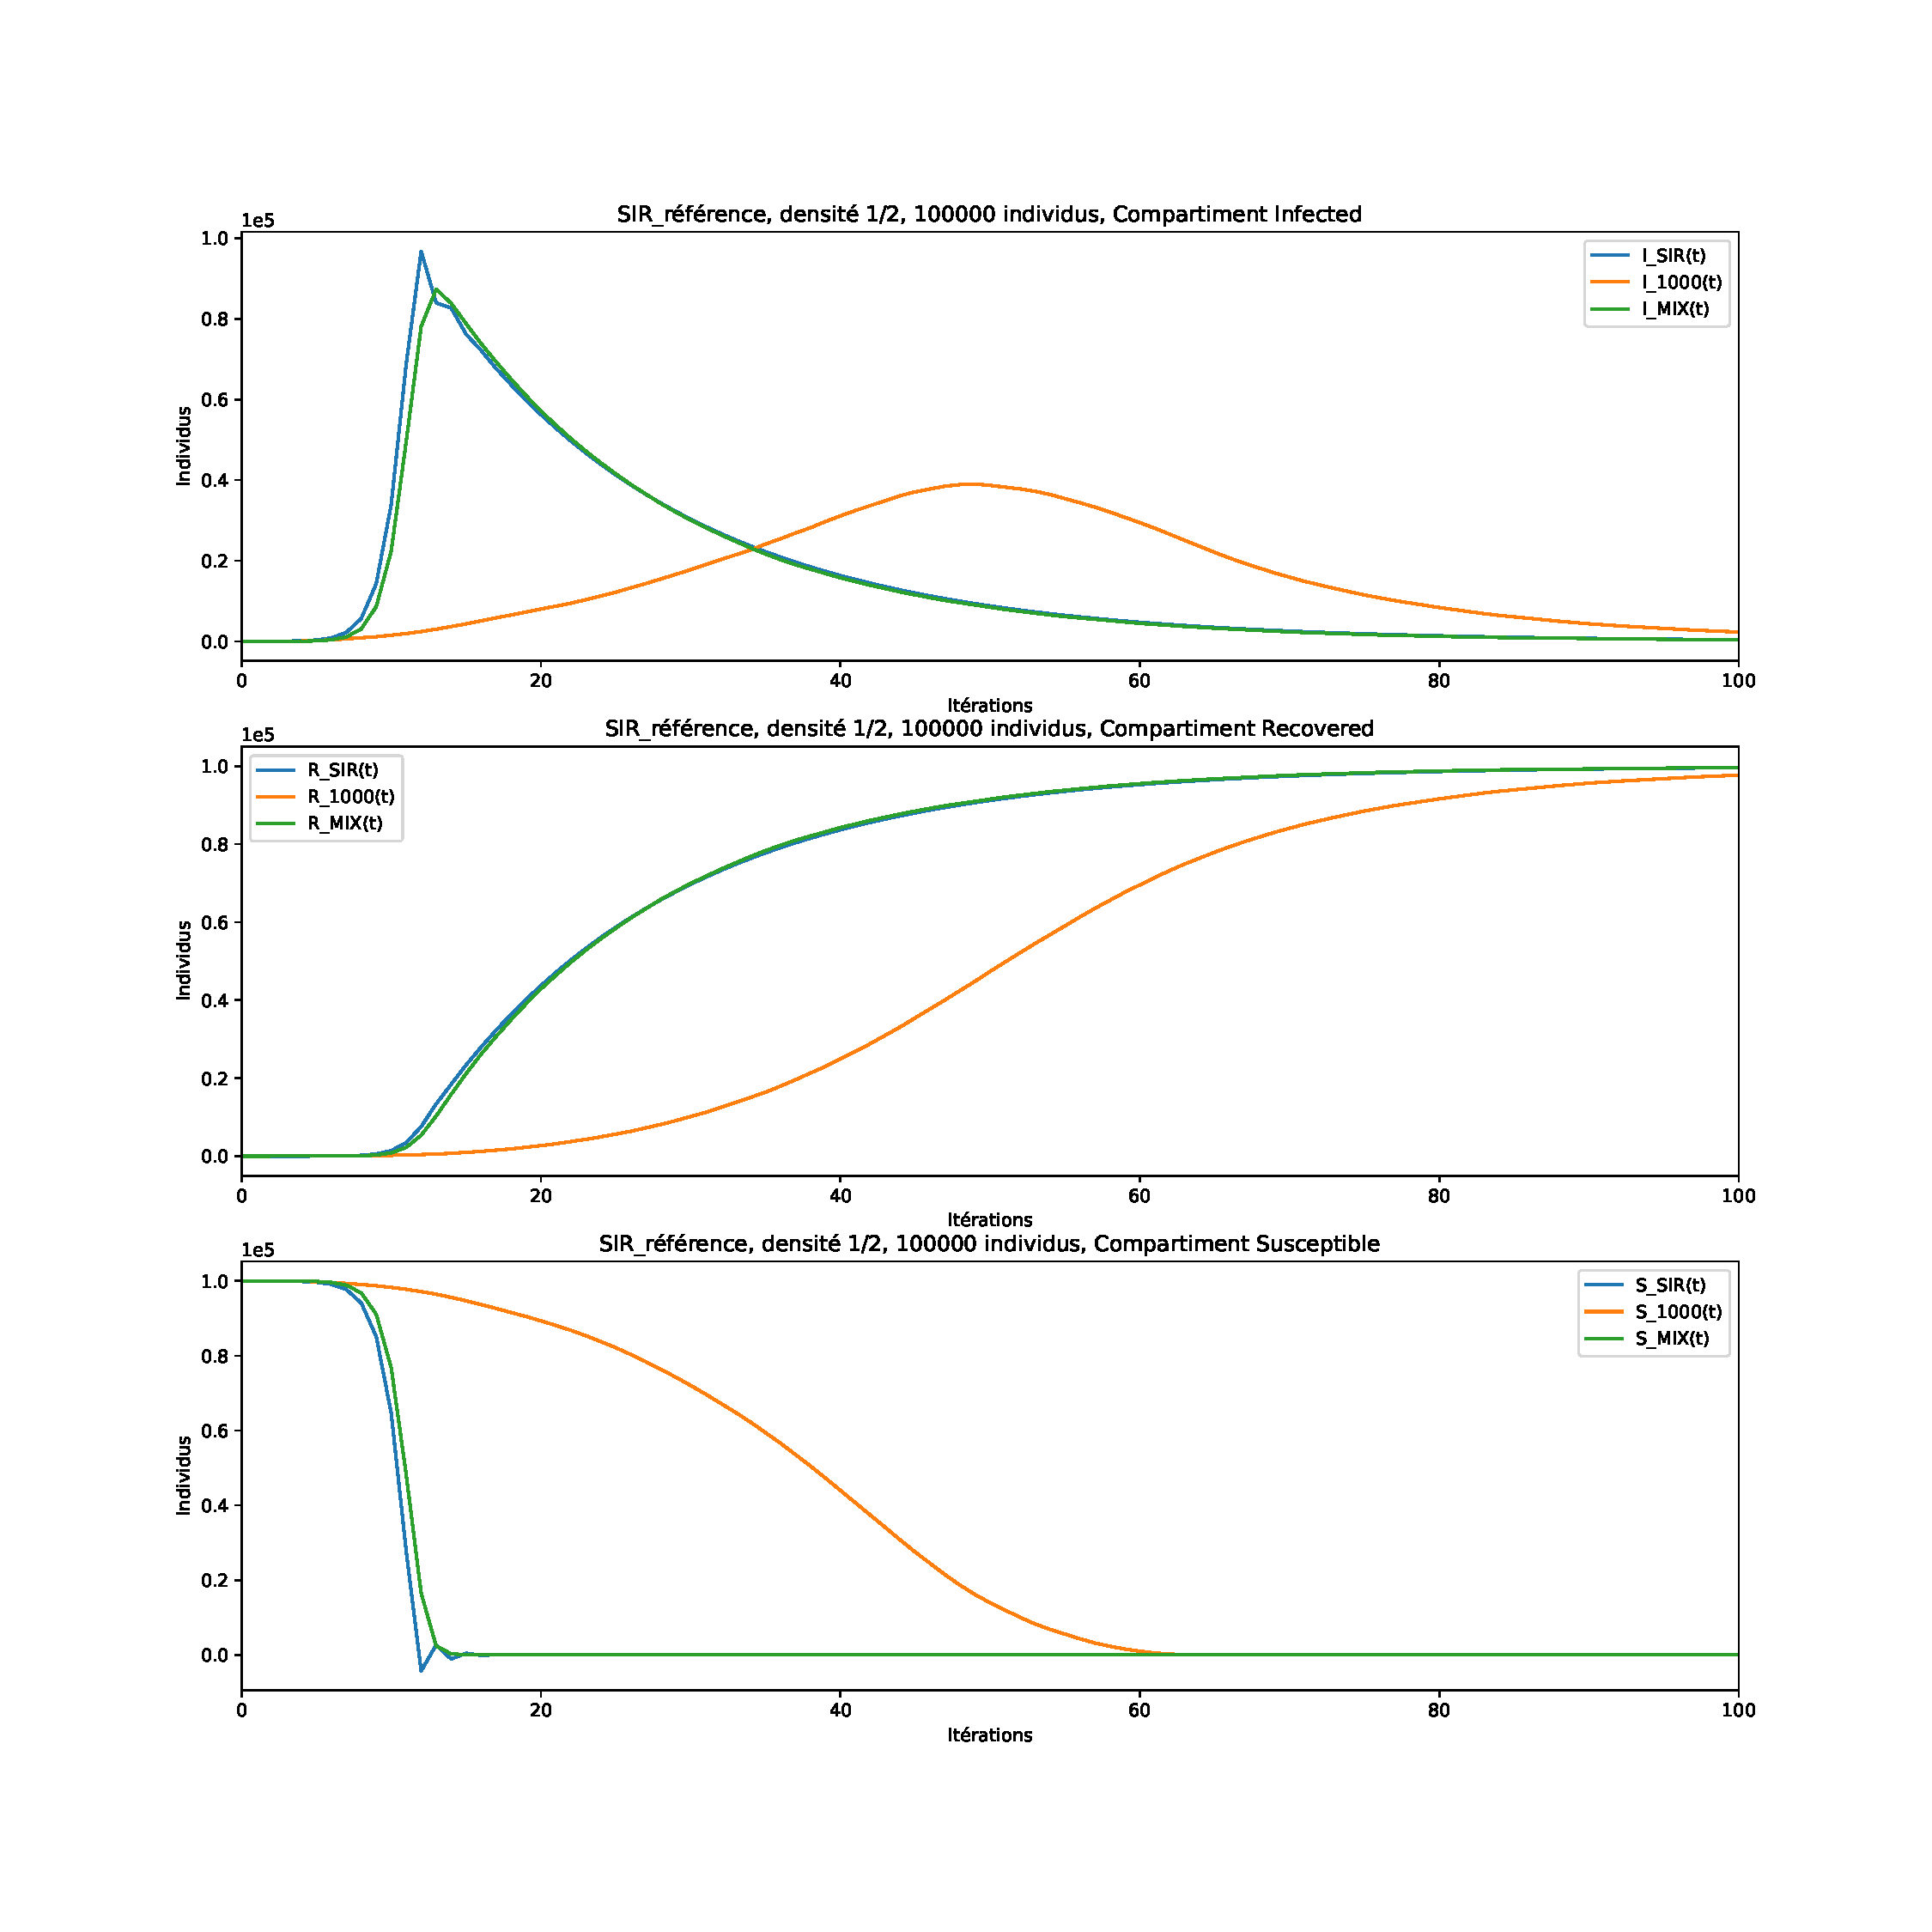
\includegraphics[width=0.9\textwidth]{Images/SIR_ref_2_100.pdf}
	\caption[Simulation SIR, densité $1/2$]{Simulations de SIR en densité $1/2$ avec une population de $100000$ individus. Chaque figure représente un compartiment avec en premier le compartiment $I$, puis $R$ et finalement $S$. Les courbes bleues représentent le modèle mathématique SIR, les vertes les simulations au mélange parfait et les oranges les simulations aux $1000$ mouvements.}
\end{figure}

Pour les systèmes de forte densité, les simulations aux $1000$ mouvements peinent à se mélanger. Par conséquent, les événements sont plus tardifs. Nous pouvons observer les mêmes comportements que pour les simulations SI.

\newpage

\begin{figure}[h]
	\centering
	\captionsetup{justification=centering}
	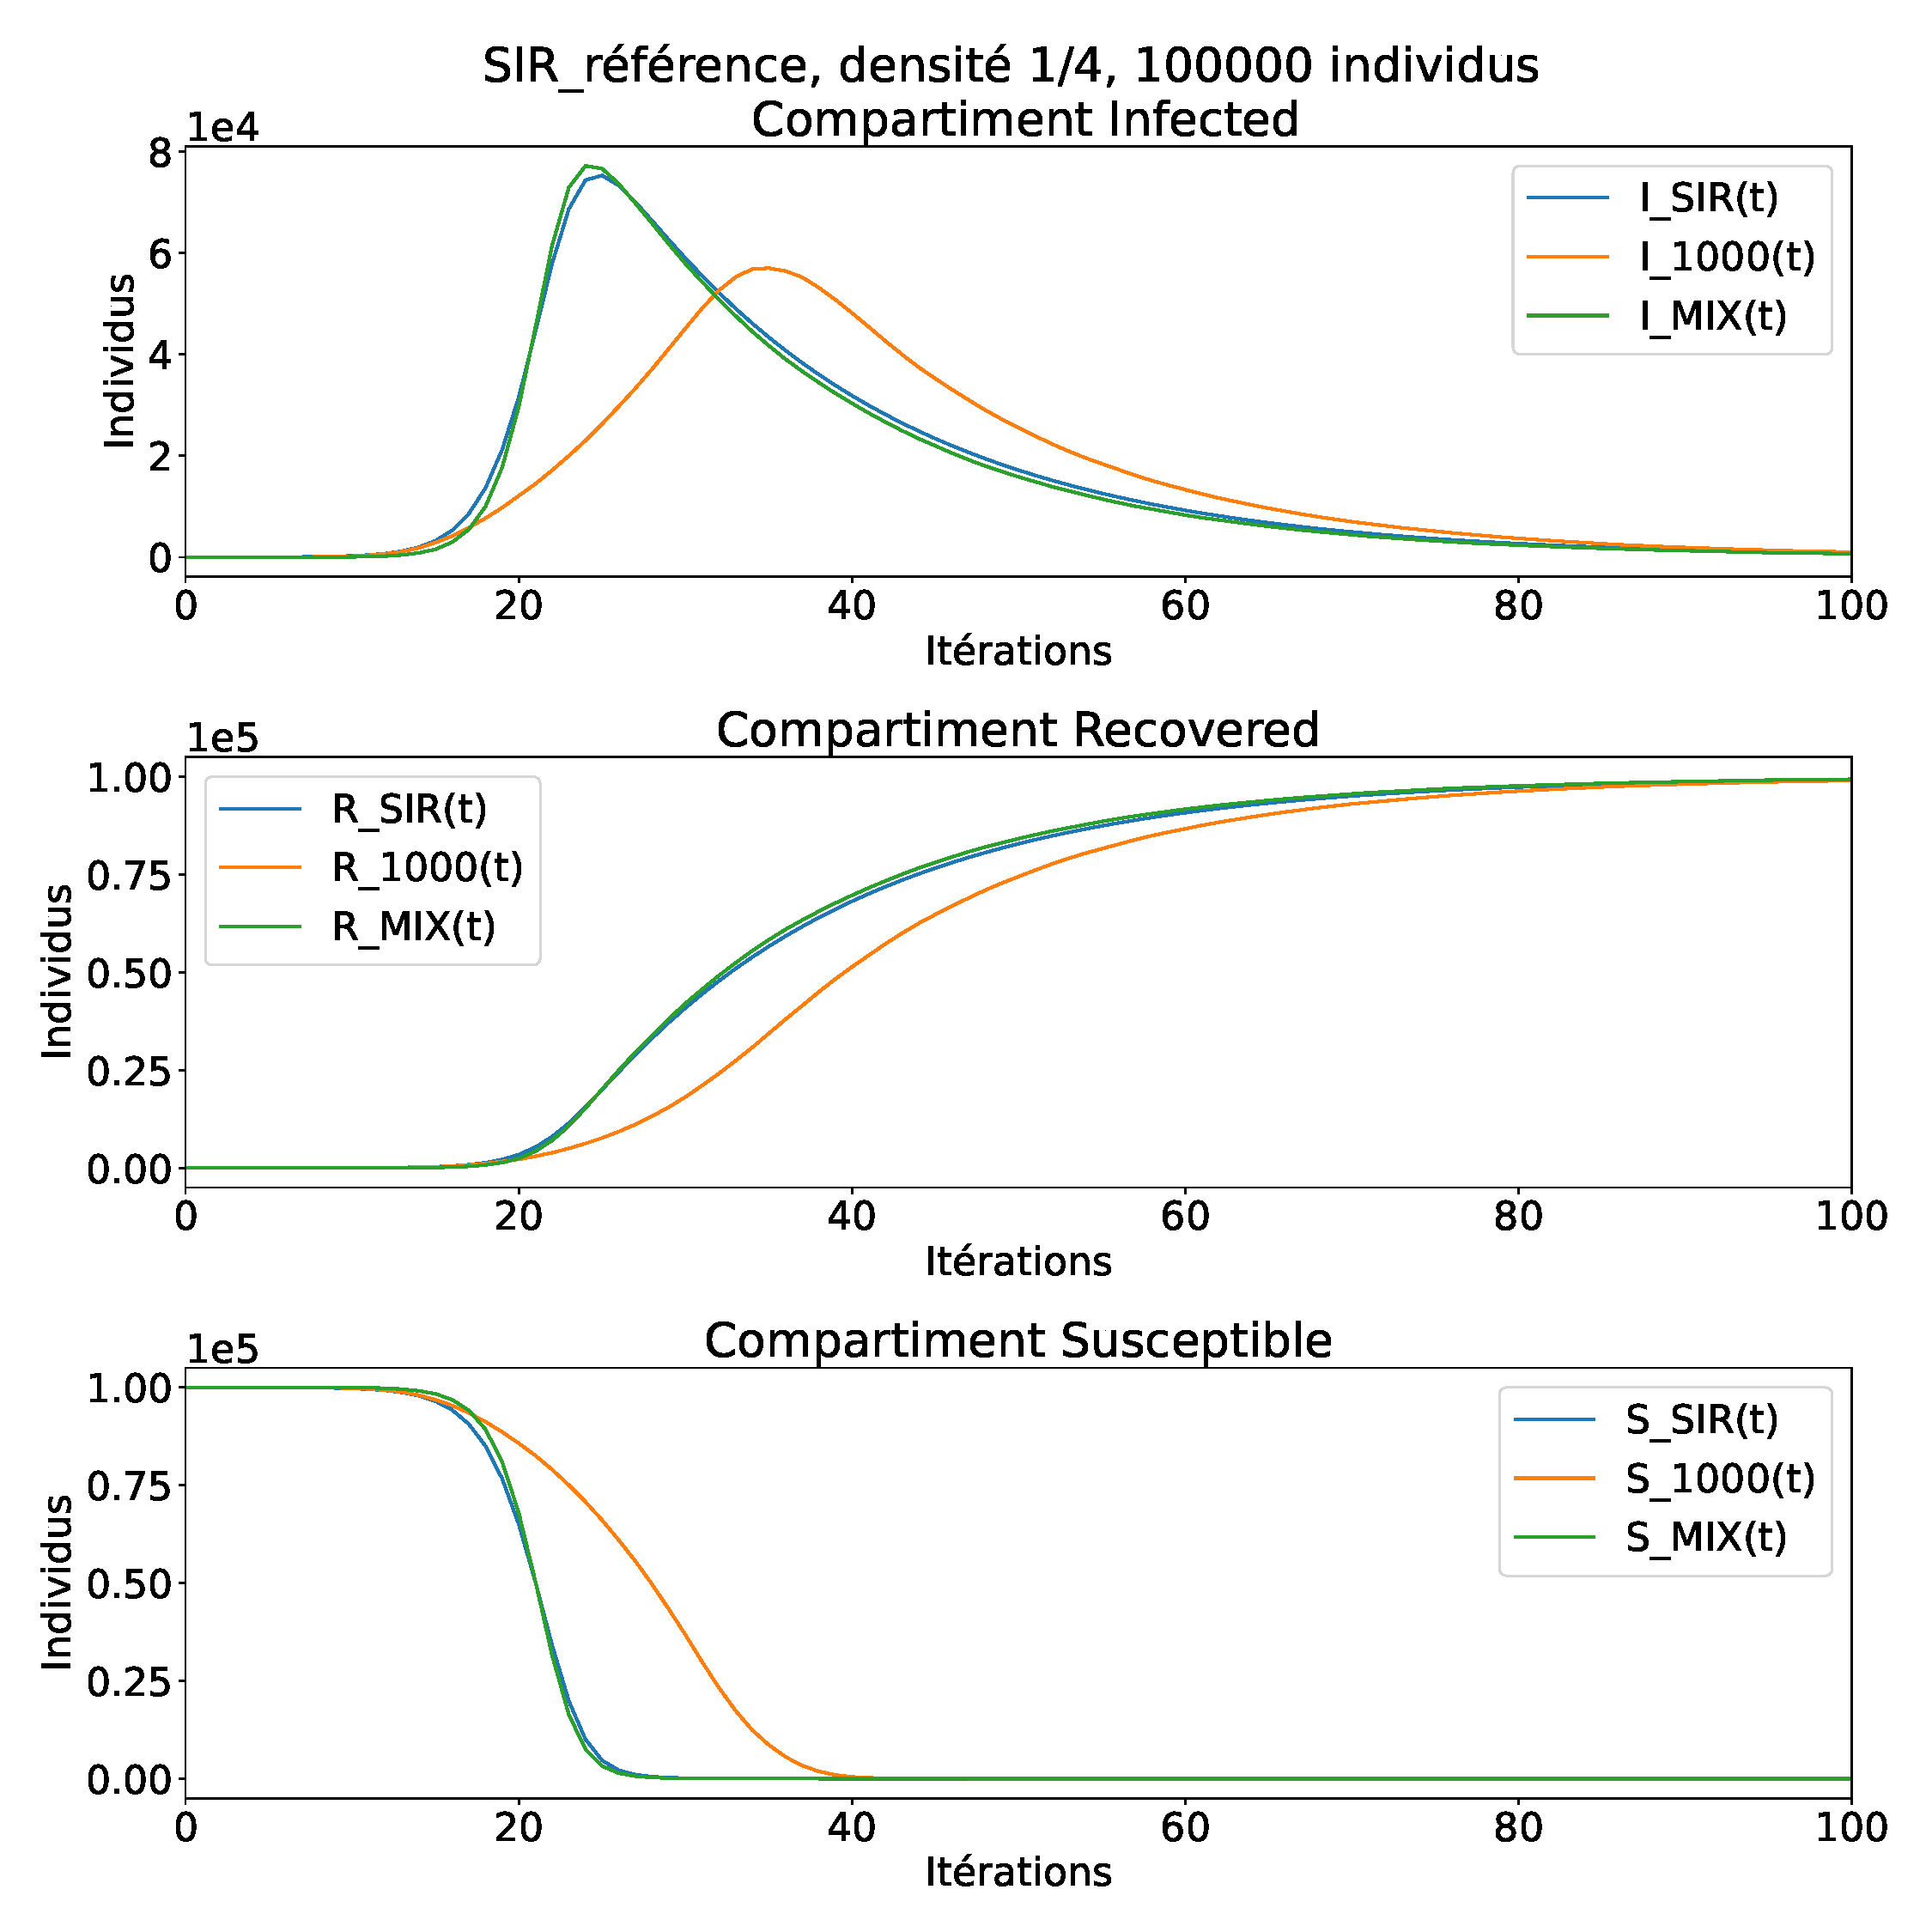
\includegraphics[width=.9\textwidth]{Images/SIR_ref_4_100.pdf}
	\caption[Simulation SIR, densité $1/4$]{Simulations de SIR en densité $1/4$ avec une population de $100000$ individus. Chaque figure représente un compartiment avec en premier le compartiment $I$, puis $R$ et finalement $S$. Les courbes bleues représentent le modèle mathématique SIR, les vertes les simulations au mélange parfait et les oranges les simulations aux $1000$ mouvements.}
\end{figure}

En densité $\frac{1}{4}$ les simulations des $1000$ mouvements tendent davantage vers le mélange parfait. Les courbes sont toujours plus progressives et donc les événements plus lents.

\newpage

\begin{figure}[h]
	\centering
	\captionsetup{justification=centering}
	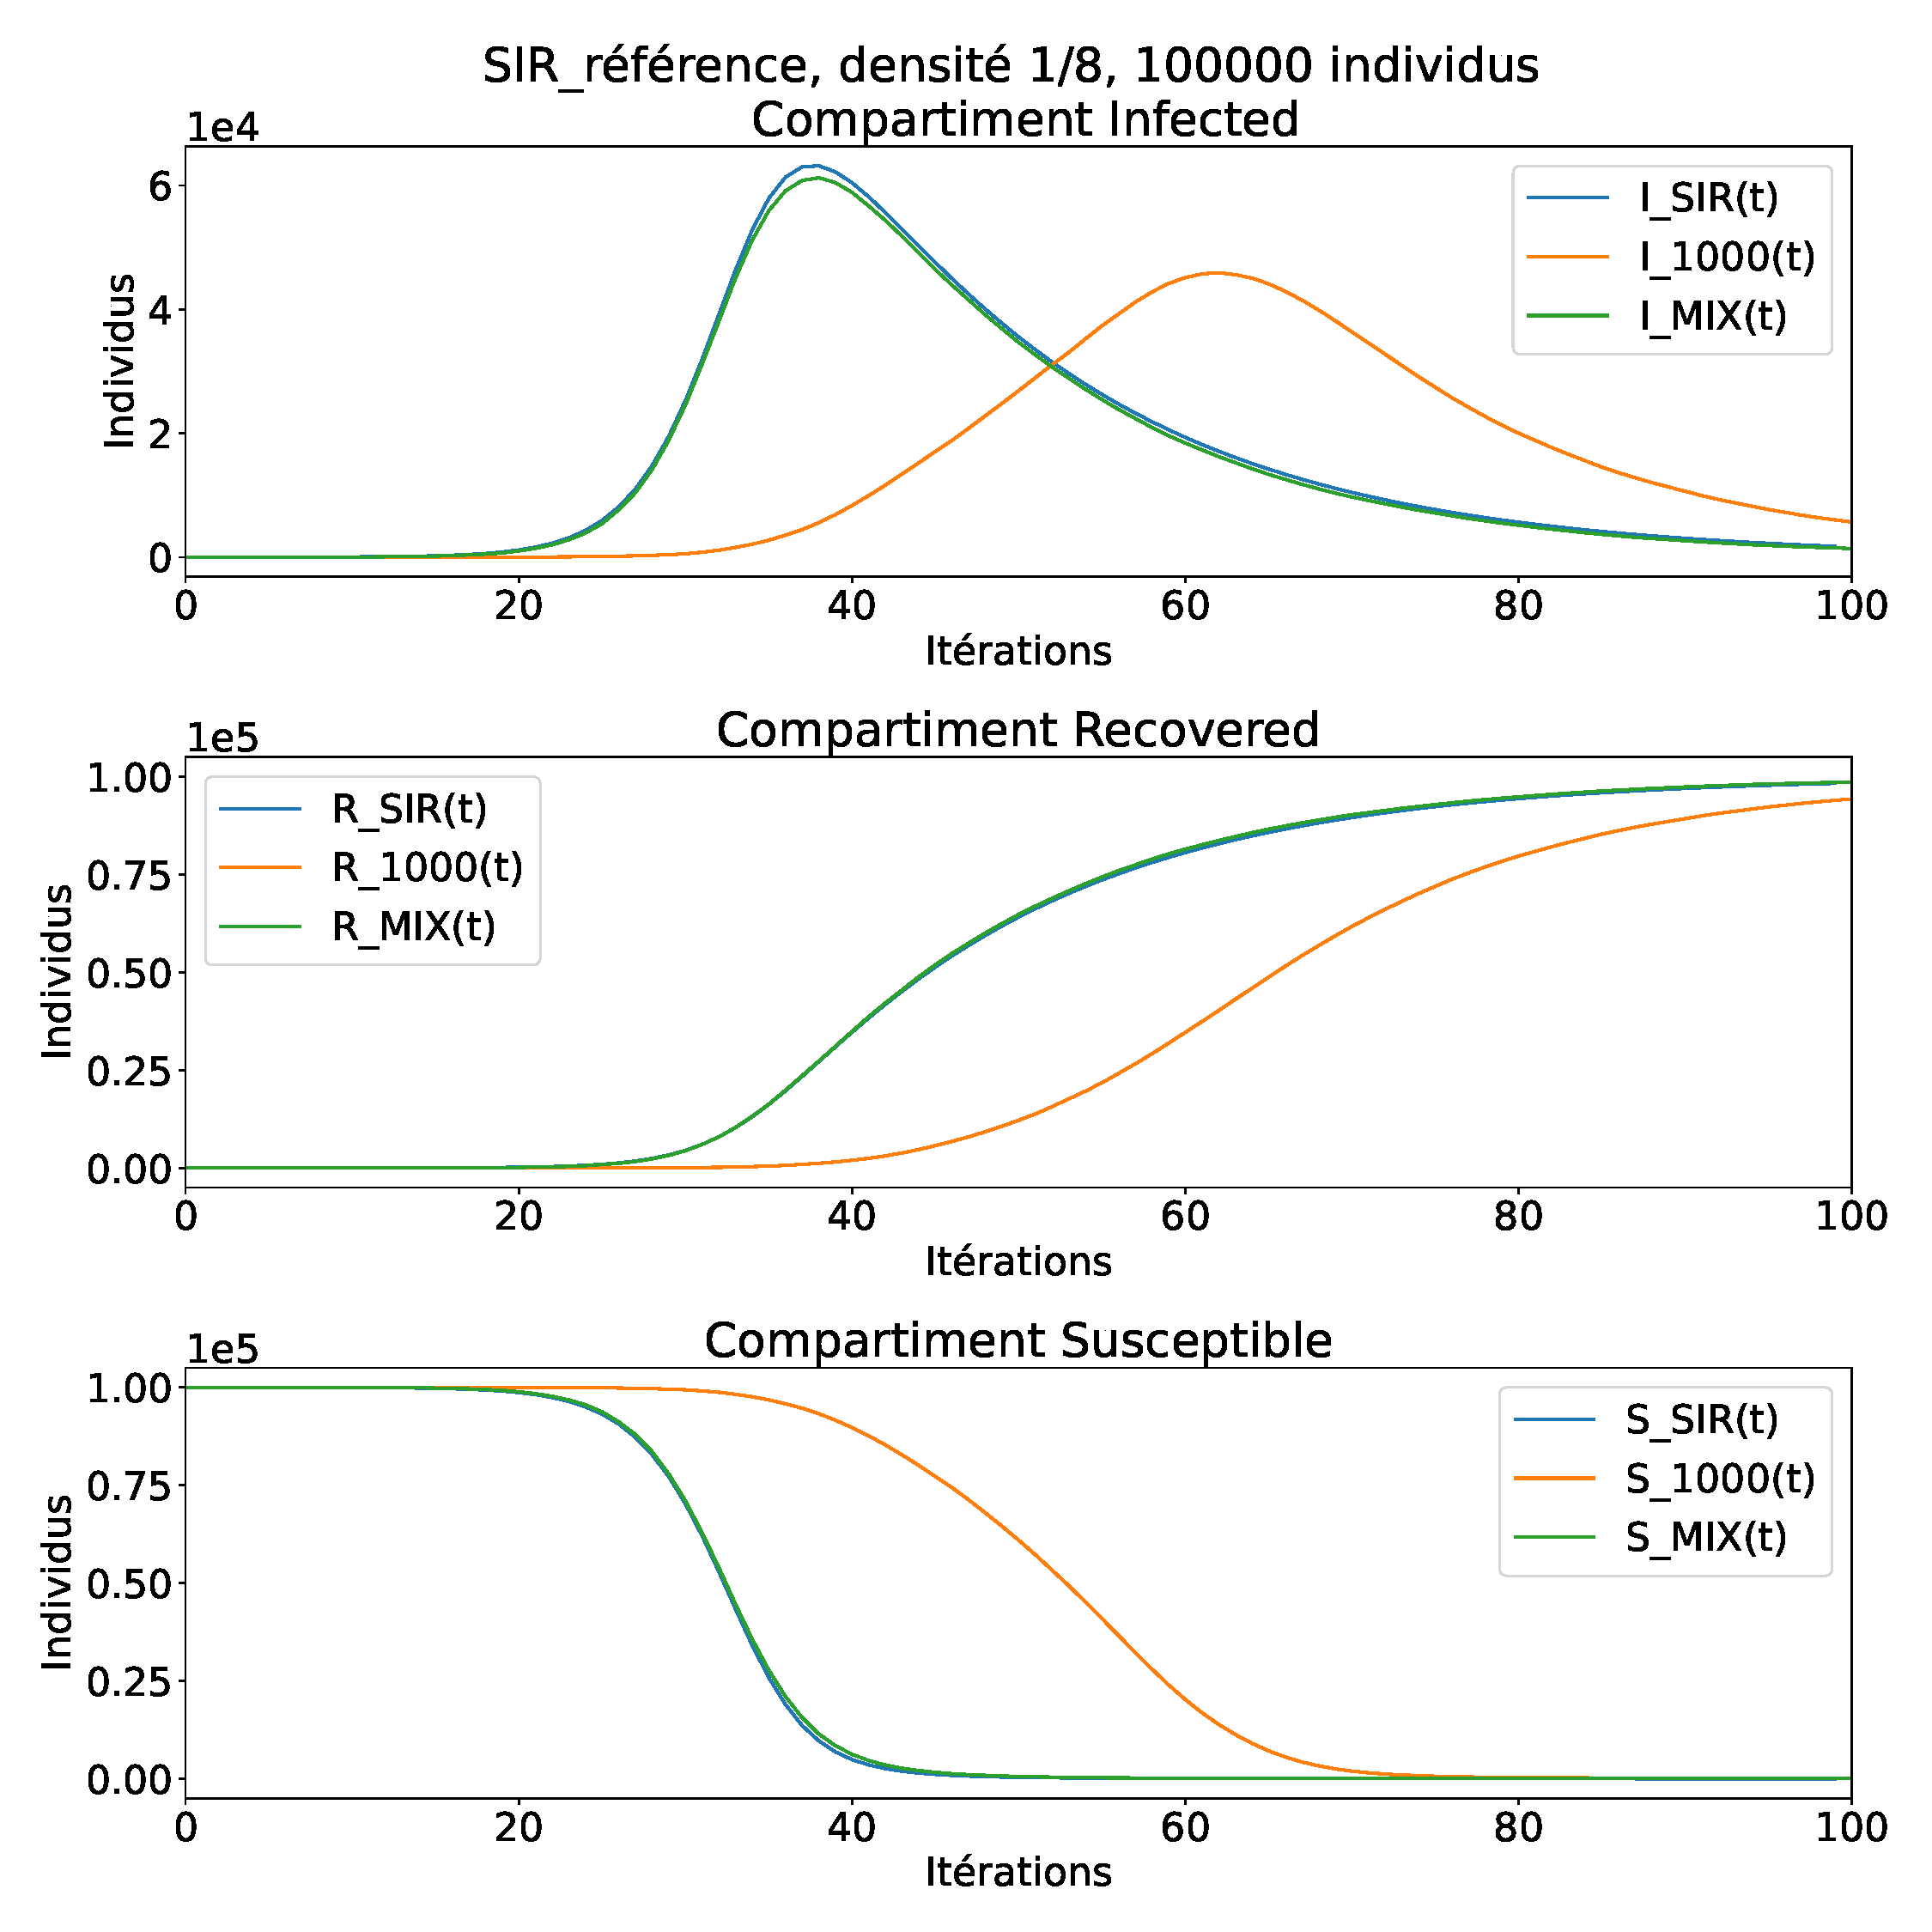
\includegraphics[width=.9\textwidth]{Images/SIR_ref_8_100.pdf}
	\caption[Simulation SIR, densité $1/8$]{Simulations de SIR en densité $1/8$ avec une population de $100000$ individus. Chaque figure représente un compartiment avec en premier le compartiment $I$, puis $R$ et finalement $S$. Les courbes bleues représentent le modèle mathématique SIR, les vertes les simulations au mélange parfait et les oranges les simulations aux $1000$ mouvements.}
\end{figure}

En plus de retrouver les mêmes comportements qu'observés précédemment, il y a un nouveau phénomène que nous pouvons observer sur les simulations en densité $1/8$. Ce phénomène est particulièrement présent sur la simulations à $5000$ individus. Nous remarquons que la croissance des courbes pour les simulations de mélange parfait sont plus rapides que le modèle mathématique SIR. Ce comportement est dû au fait que nos simulations peuvent nécessiter d'un temps de latence avant l'émergence d'un événement. Alors qu'au contraire le modèle SIR n'est pas victime de cette latence.\\

Par conséquent, pour joindre le modèle SIR aux simulations il faut prendre en compte le temps de latence des simulations. Ce temps de latence est particulièrement présent sur les systèmes peu denses car dans ces configurations les pandémies peuvent prendre du temps à apparaitre. Ce phénomène est étudié dans un autre chapitre.

\newpage

\begin{figure}[h]
	\centering
	\captionsetup{justification=centering}
	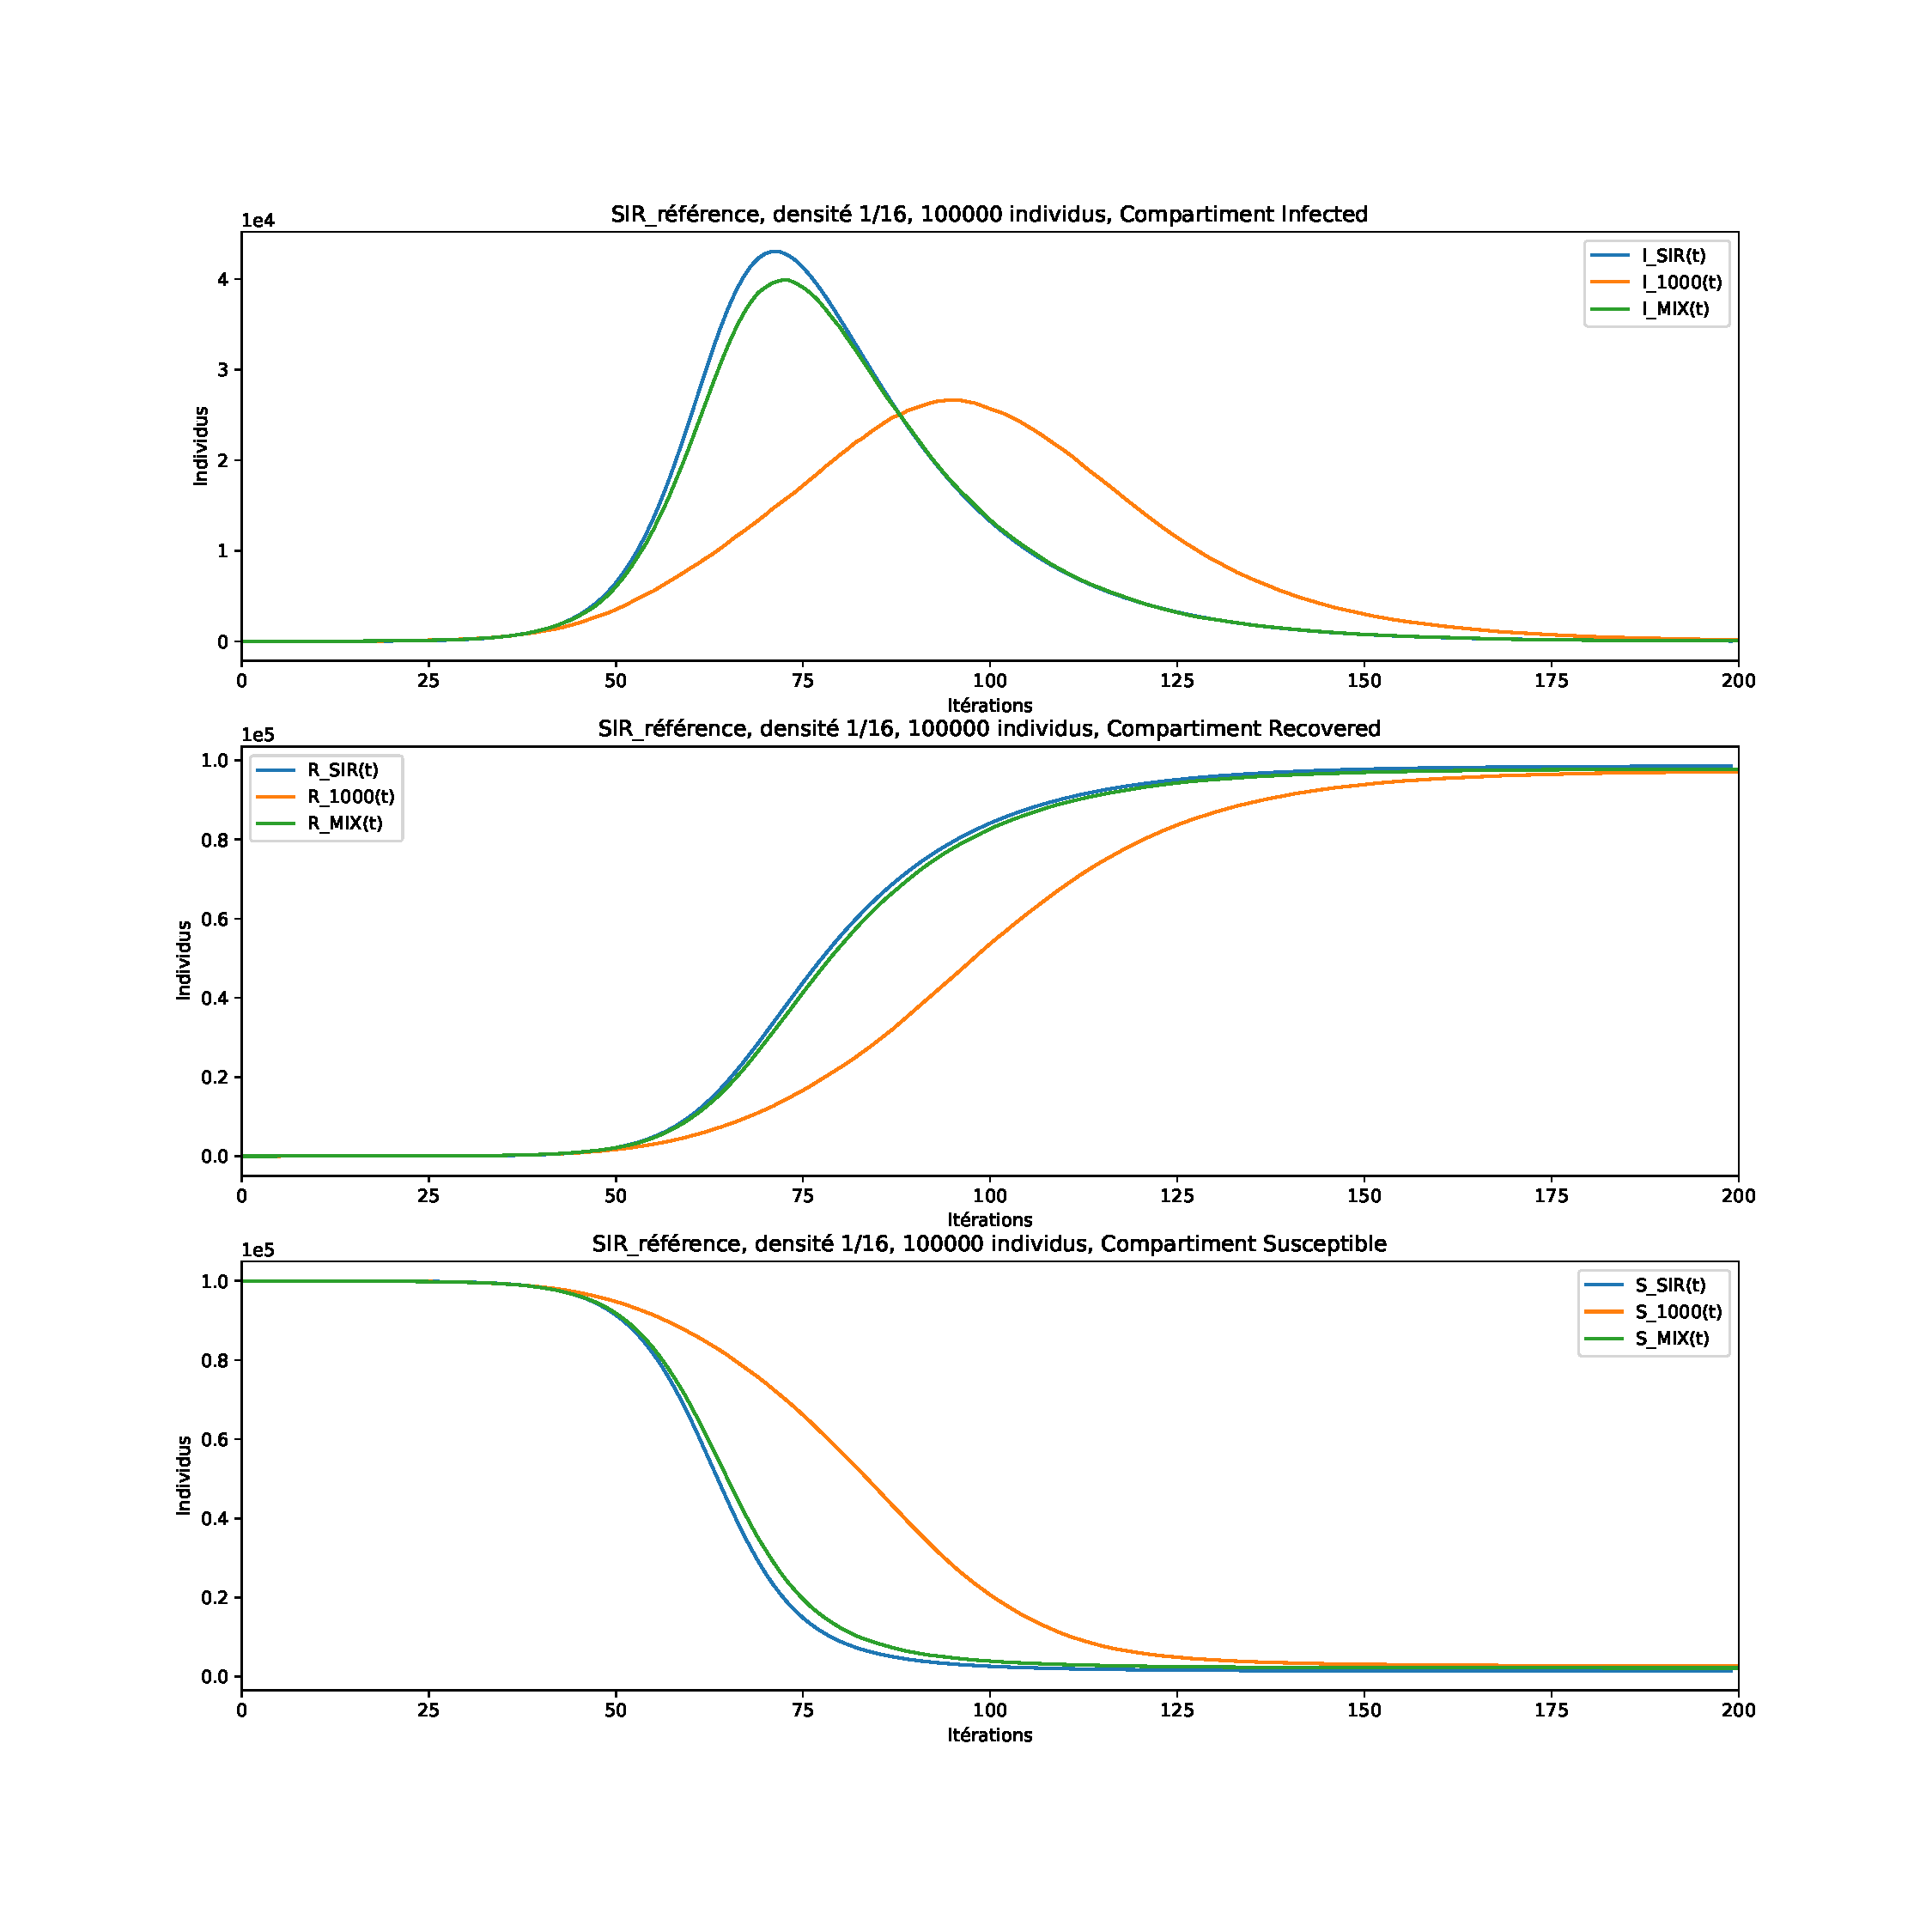
\includegraphics[width=.9\textwidth]{Images/SIR_ref_16_100.pdf}
	\caption[Simulation SIR, densité $1/16$]{Simulations de SIR en densité $1/16$ avec une population de $100000$ individus. Chaque figure représente un compartiment avec en premier le compartiment $I$, puis $R$ et finalement $S$. Les courbes bleues représentent le modèle mathématique SIR, les vertes les simulations au mélange parfait et les oranges les simulations aux $1000$ mouvements.}
\end{figure}

Malgré des observations déjà analysées, nous observons des oscillations sur la simulation à $5000$ indiviuds. Ce phénomène n'était pas présent sur les simulations SI et ceci à cause de l'absense du compartiment $Recovered$. Deux raisons explique ce comportement, le premier est que le mécanisme d'immunisation transfert des individus du compartiment $I$ au $R$ et donc abaisse la courbe du compartiment $I$. Le second est dû à la densité du système qui est très faible, par conséquent il y a peu de contactes qui s'effectuent ce qui crée des oscillations. Ces oscillations sont aussi présentes sur des sytèmes plus denses mais pas perceptibles car moyennée par un grand nombre d'événements.

\section{Analyses}

\subsection{Mean Absolute Error}

Le mean absolute error permet de quantifier les différences entre les simulations et le modèle mathématique SIR. Les calculs suivants ont été effectués sur les simulations au mélnage parfait. Contrairement au modèle SI, le modèle SIR contient trois courbes différentes par conséquent chacune de ces courbes a sont propre MAE. Le tableau ci-dessous donne la moyenne de ces trois résultats et ceci pour toutes les simulations SIR.

\begin{table}[H]
	\centering
	\captionsetup{justification=centering}
	\caption[Mean Aboslute Error Normalized : SIR]{Mean Aboslute Error Normalized : Calcul des erreurs entre les simulations au mélange parfait et le modèle mathématique SIR sur $4$ niveaux de densités et $4$ niveaux de populations. Les valeurs sont les moyennes des MAE de chaque compartiment et le résultat est divisé par la taille de la population.\label{tab:grid}}
	\begin{tabular}{@{\extracolsep{\fill} } c|| c| c| c| c|}
		     & 5000                & 20000               & 50000               & 100000              \\
		\midrule
		\midrule
		1/2  & $4.3\mathrm{e}{-3}$ & $2.1\mathrm{e}{-3}$ & $2.7\mathrm{e}{-3}$ & $2.5\mathrm{e}{-3}$ \\
		\midrule
		1/4  & $3.8\mathrm{e}{-3}$ & $3.0\mathrm{e}{-3}$ & $2.1\mathrm{e}{-3}$ & $2.6\mathrm{e}{-3}$ \\
		\midrule
		1/8  & $9.6\mathrm{e}{-3}$ & $2.8\mathrm{e}{-3}$ & $1.9\mathrm{e}{-3}$ & $2.3\mathrm{e}{-3}$ \\
		\midrule
		1/16 & $8.5\mathrm{e}{-3}$ & $3.2\mathrm{e}{-3}$ & $6.2\mathrm{e}{-3}$ & $7.2\mathrm{e}{-3}$ \\
		\bottomrule
	\end{tabular}
\end{table}

Les résultats pour le modèle SIR sont généralement moins précis que pour le modèle SI. Certains résultats sont intéressant par exemple les courbes de densité $\frac{1}{8}$ avec $5000$ individus. L'erreur sur cette courbe est élevée car la simulation souffre de latence, par conséquent le déclanchement de l'événement se fait tardivement. C'est également la raison pour laquelle la simulation au $1000$ mouvements évolue plus rapidement que la simulation au mélange parfait.\\

En densité $\frac{1}{16}$ d'avantage d'erreurs apparaissent. Premièrement, une plus grande erreur de la simulation à $5000$ individus et due aux oscillations causées par le peu d'événements du système, donc les systèmes peu denses ont une plus grande erreur. Deuxièmement les simulations à faible densité prennent du temps déclancher un événement, ce qui engendre un temps de latence. Ce temps de latence est innexistant dans le modèle SIR, par conséquent notre modèle ne se comporte plus exactement comme le modèle mathématique.

\newpage

\subsection{Variations aléatoires}

Tout comme pour les simulations SI, nous calculons les variations d'une simulation à une autre et ceci pour des paramètres identiques. Les mesures sont faites sur un ensemble de simulations de densité $\frac{1}{8}$ ainsi que $\frac{1}{16}$ avec une population de $20000$ individus.

\begin{figure}[h]
	\centering
	\captionsetup{justification=centering}
	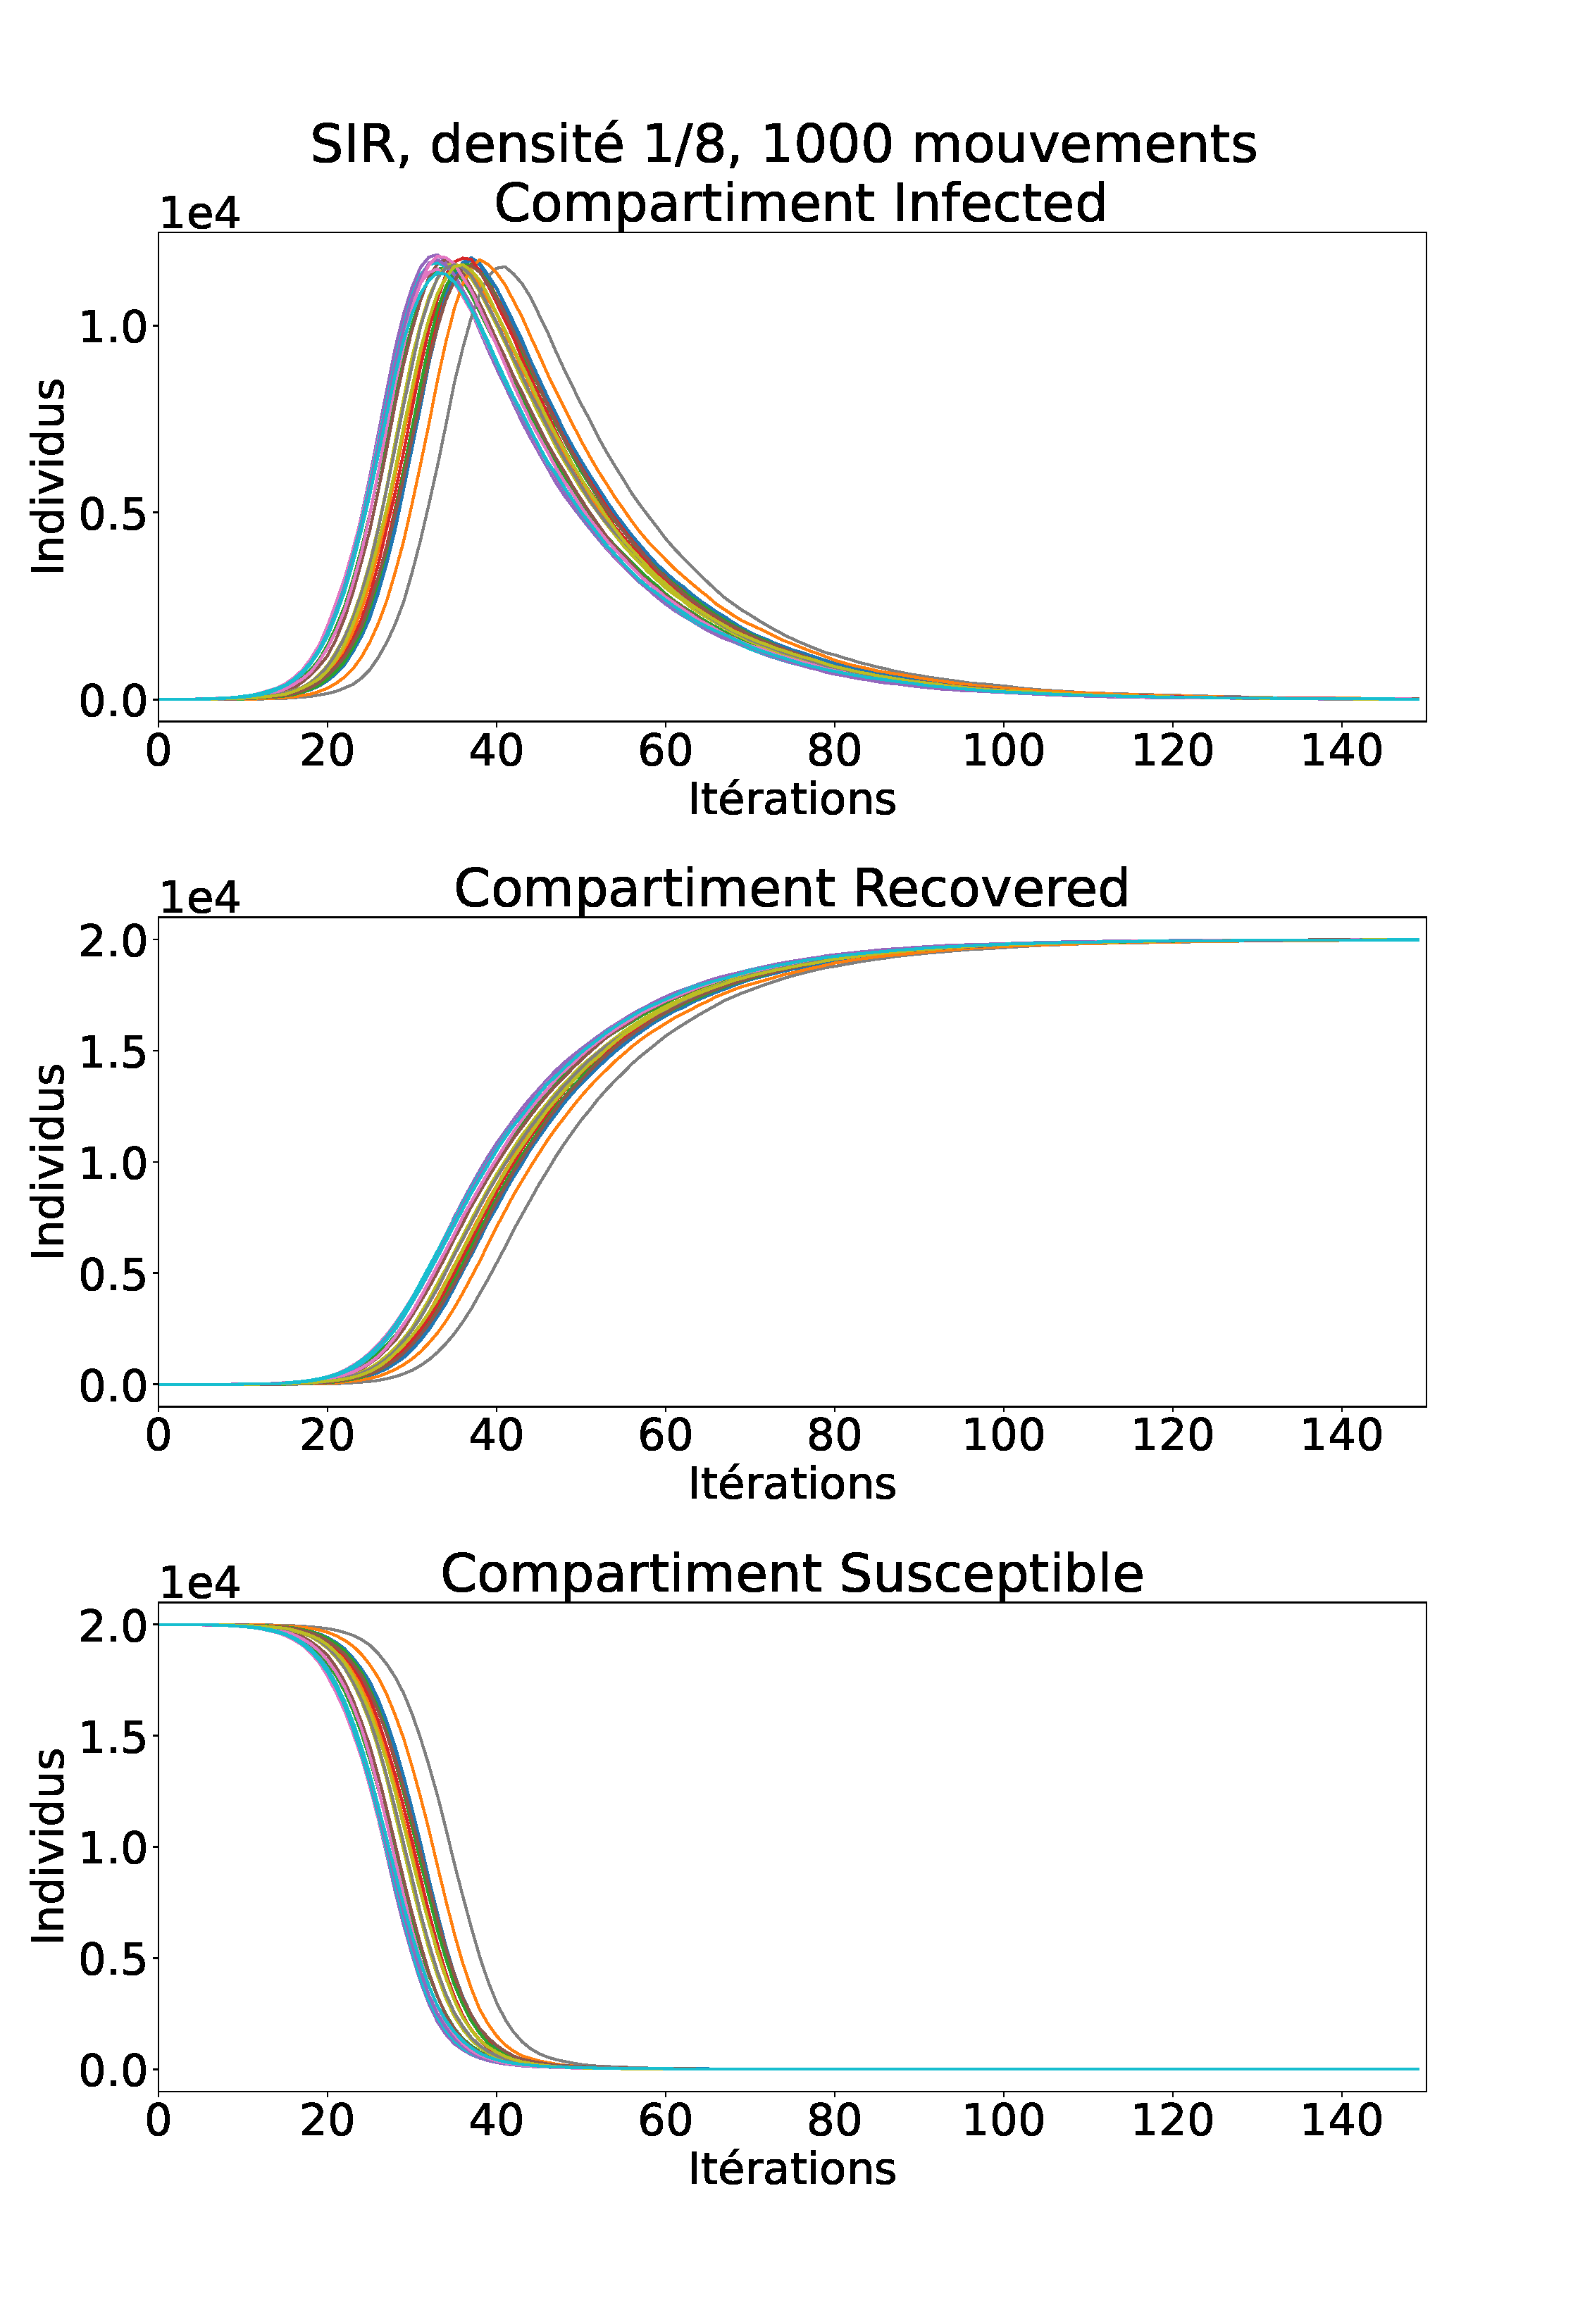
\includegraphics[width=.49\textwidth]{Images/SIR_divergence_8_1000.pdf}
	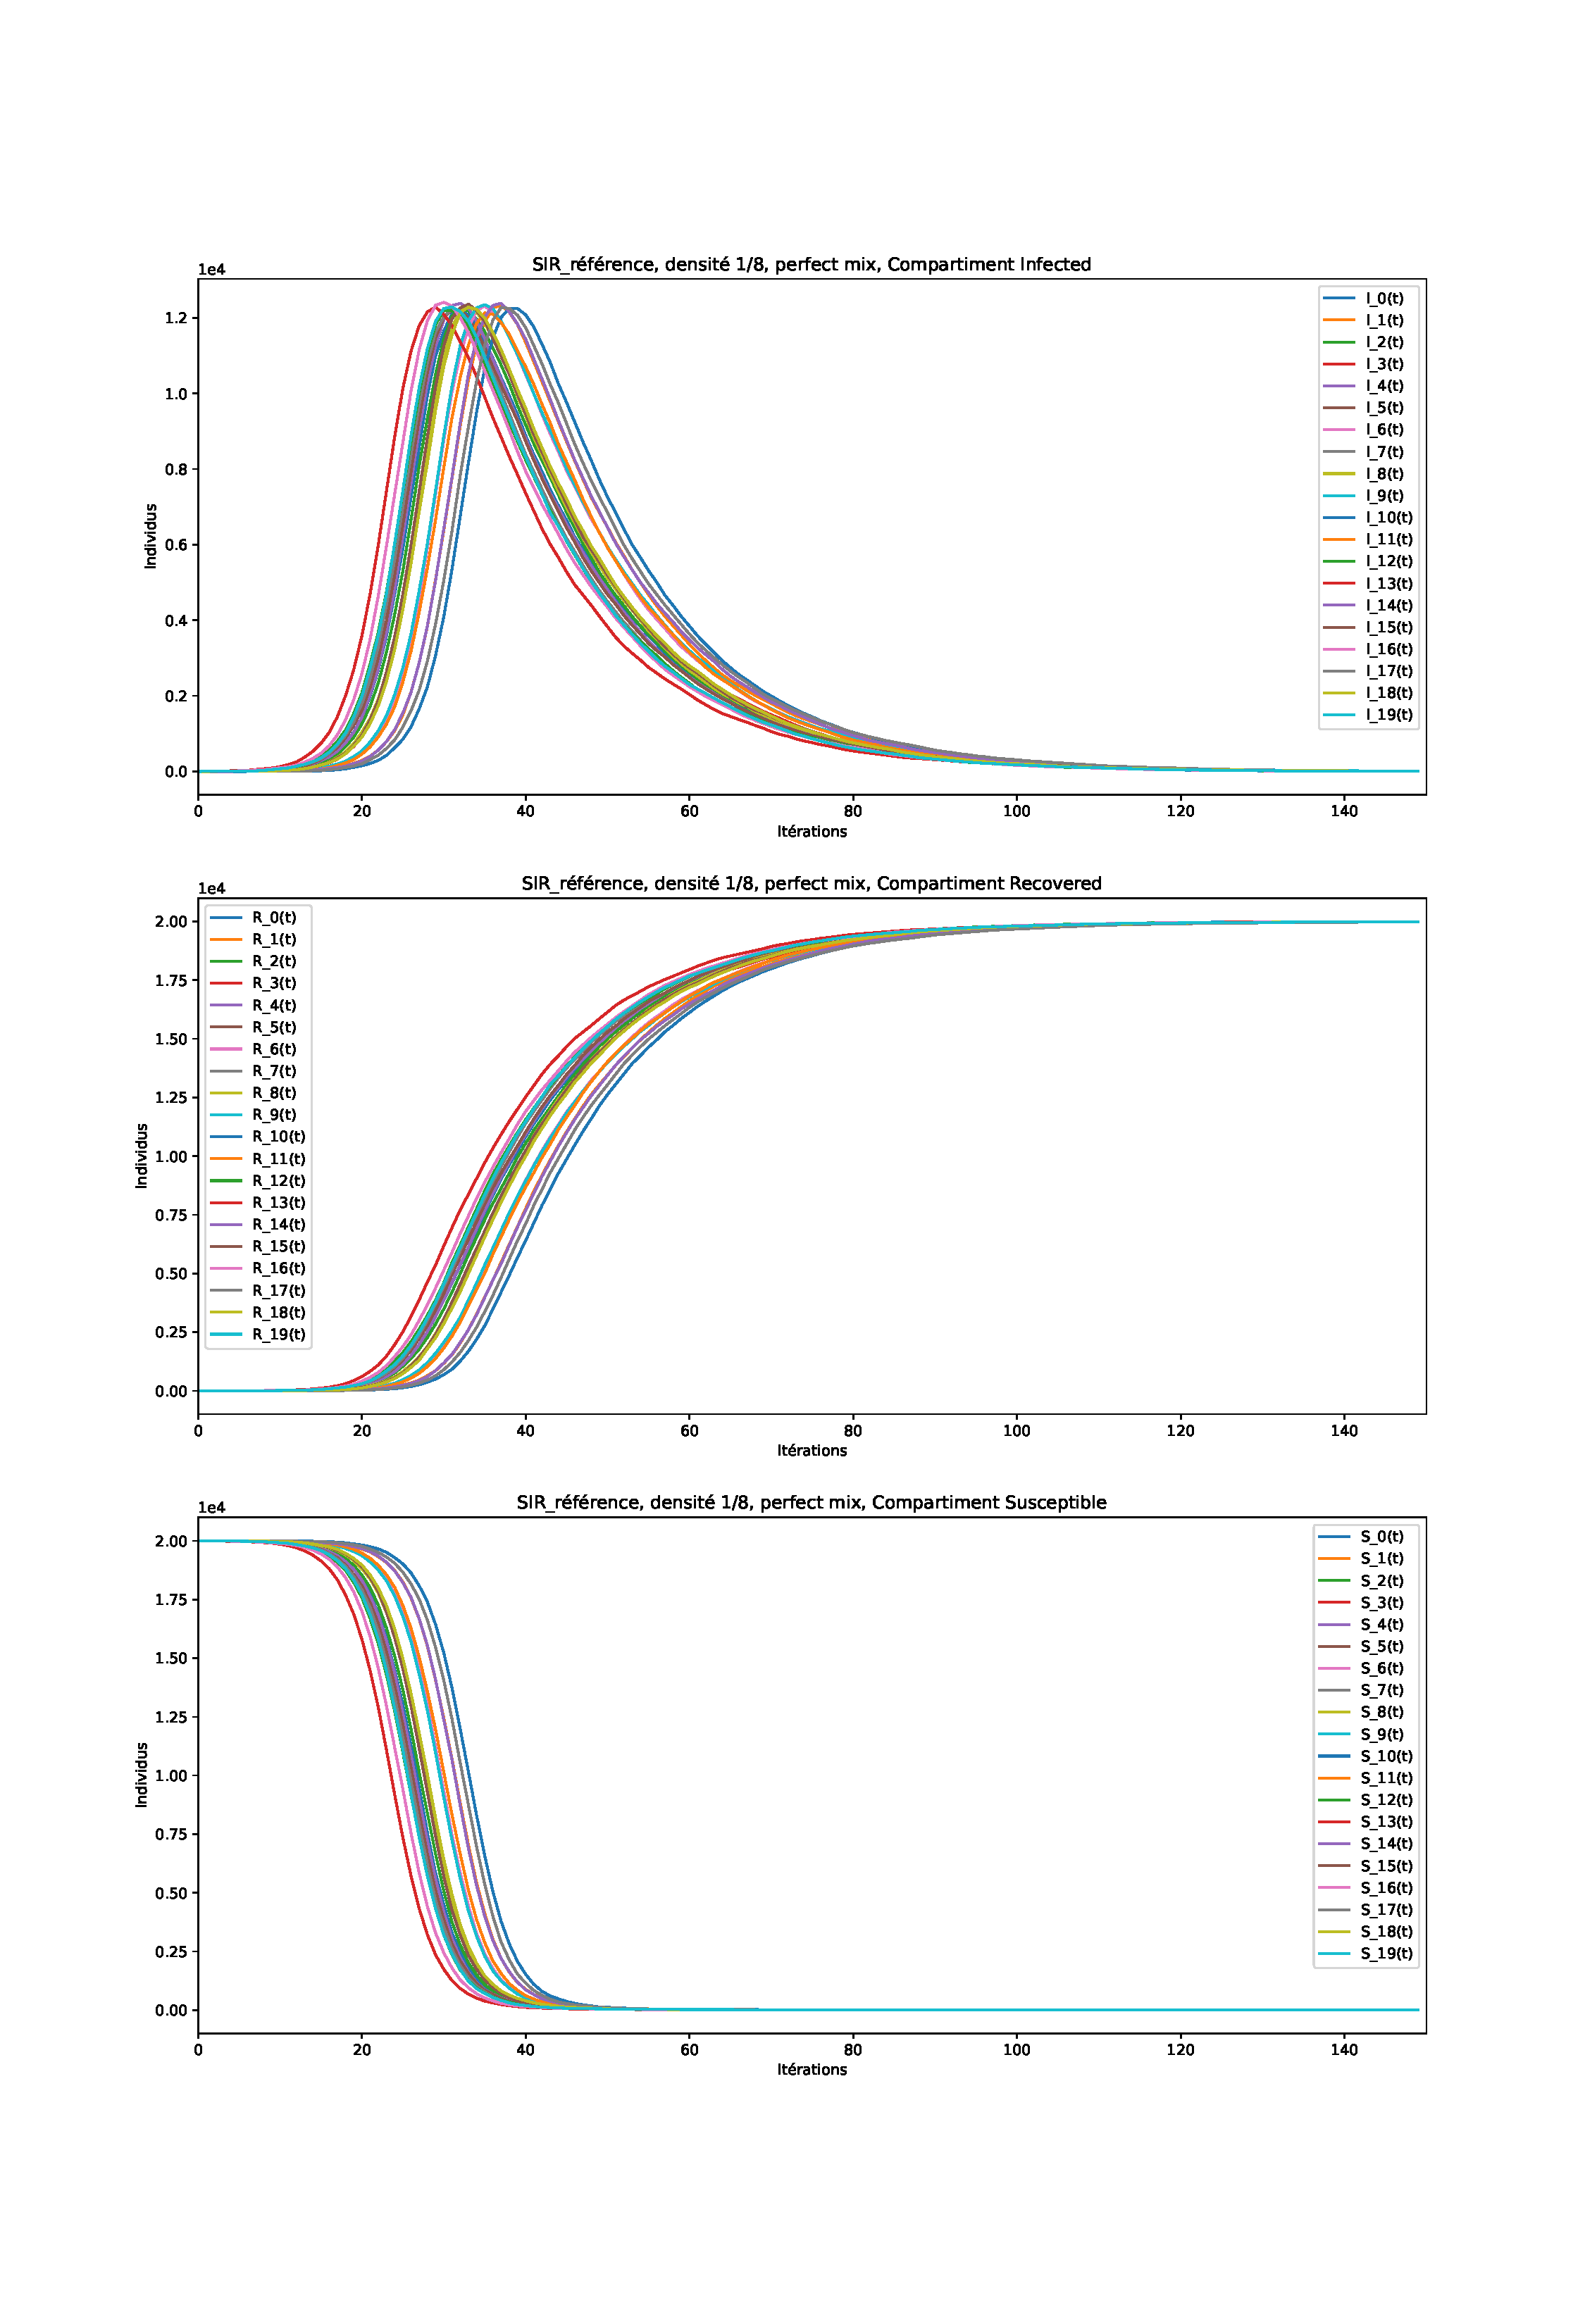
\includegraphics[width=.49\textwidth]{Images/SIR_divergence_8_mix.pdf}
	\caption[Variations SIR]{Sur la gauche nous avons des simulations en densité $1/8$ avec une populations de $20000$ individus et un mode de déplacements de $1000$ mouvements. Un ensemble de $20$ simulations y sont superposées avec des paramètres identiques. Sur la droite nous avons la même expérience sauf qu'il s'agit de simulations au mélange parfait.}
\end{figure}

Idem aux simulations SI, nous pouvons observer de grandes variations d'une simulation à une autre. A nouveau, ce sont les systèmes peu denses qui sont victimes de plus grandes variations. La mesure de la variation n'est pas la même que pour le modèle SI. Ici nous mesurons l'itération du pic de contaminés simultanés, c'est-à-dire l'itération de la valeur maximale des courbes du compartiment $Infected$.\\

Les analyses permettent de calculer la moyenne ainsi que la variance. 

\begin{table}[H]
	\centering
	\captionsetup{justification=centering}
	\caption[Variations aléatoires : SIR]{Calcul des variations aléatoires sur $20$ simulations identiques. La mesures est prise pour les deux modes de mouvements ainsi que pour deux densités lorque le maximum dans le compartiment $I$ est atteint. La mesure du minimum décrit la simulation la plus rapide et le maximum décrit la plus lente. La moyenne ainsi que l'écart à la moyenne est aussi calculé.\label{tab:grid}}
	\begin{tabular}{@{\extracolsep{\fill} } c|| c| c| c| c|}
		        & \multicolumn{2}{|c|}{1000 mouvements} & \multicolumn{2}{|c|}{Mélange parfait}                    \\
		\midrule
		densité & 1/8                                   & 1/16                                  & 1/8    & 1/16    \\
		\midrule
		\midrule
		min     & $33$                                  & $62$                                  & $29$   & $59$    \\
		\midrule
		max     & $41$                                  & $93$                                  & $38$   & $87$    \\
		\midrule
		mean    & $35.35$                               & $72.85$                               & $33.2$ & $69.35$ \\
		\midrule
		std     & $2.10$                                & $7.28$                                & $2.58$ & $6.77$  \\
		\bottomrule
	\end{tabular}
\end{table}

Le tableau confirme plusieurs attentes du modèle. Premièrement, les simulations au mélange parfait sont plus rapides que les simulations aux $1000$ mouvements et ceci pour les deux densités étudiées. Deuxièmement, la moyenne des déviations est plus grande sur des systèmes moins denses, ce qui confirme nos hypothèses.

\subsection{Latence des simulations}

Certaines simulations du modèle implémenté divergent du modèle SIR. Une des hypothèse expliquant ce phénomène est que les simulations peuvent nécessiter d'un certain temps de latence avant que la pandémie apparaisse, une période durant laquelle la situation n'évolue pas. Cette latence est théoriquement possible dans notre modèle par contre elle est inexistante dans le modèle mathématique SIR.\\

L'objectif de cette section est de déterminer l'impacte de la latence sur le "mean absolute error" entre les simulations et le modèle mathématique SIR. Pour ce faire nous utilisons une simulation qui semble subir de la latence. De toutes les simulations du document, peu d'entre elle montrent des signes de latence. Ceci est compréhensible car la latence croît avec la diminution de la denstié des système mais décrôit en même temps. Un système à faible densité a une certaine latence à cause du manque d'événements mais en même temps le manque d'événements réduit la latence car la progression de la pandémie en sera ralentie et donc SIR s'adaptera mieux à la simulation.\\

\newpage 

Par conséquent, la latence est généralement peu présente dans les simulations car le phénomène est auto-compensé. La simulation ci-dessous est l'exemple le plus explicite du comportement. La densité de cette simulation est de $\frac{1}{8}$ ce qui semble être une densité qui révèle de la latence. Tous les systèmes plus ou moins denses du document n'ont pas donné autant de latence.

\begin{figure}[h]
	\centering
	\captionsetup{justification=centering}
	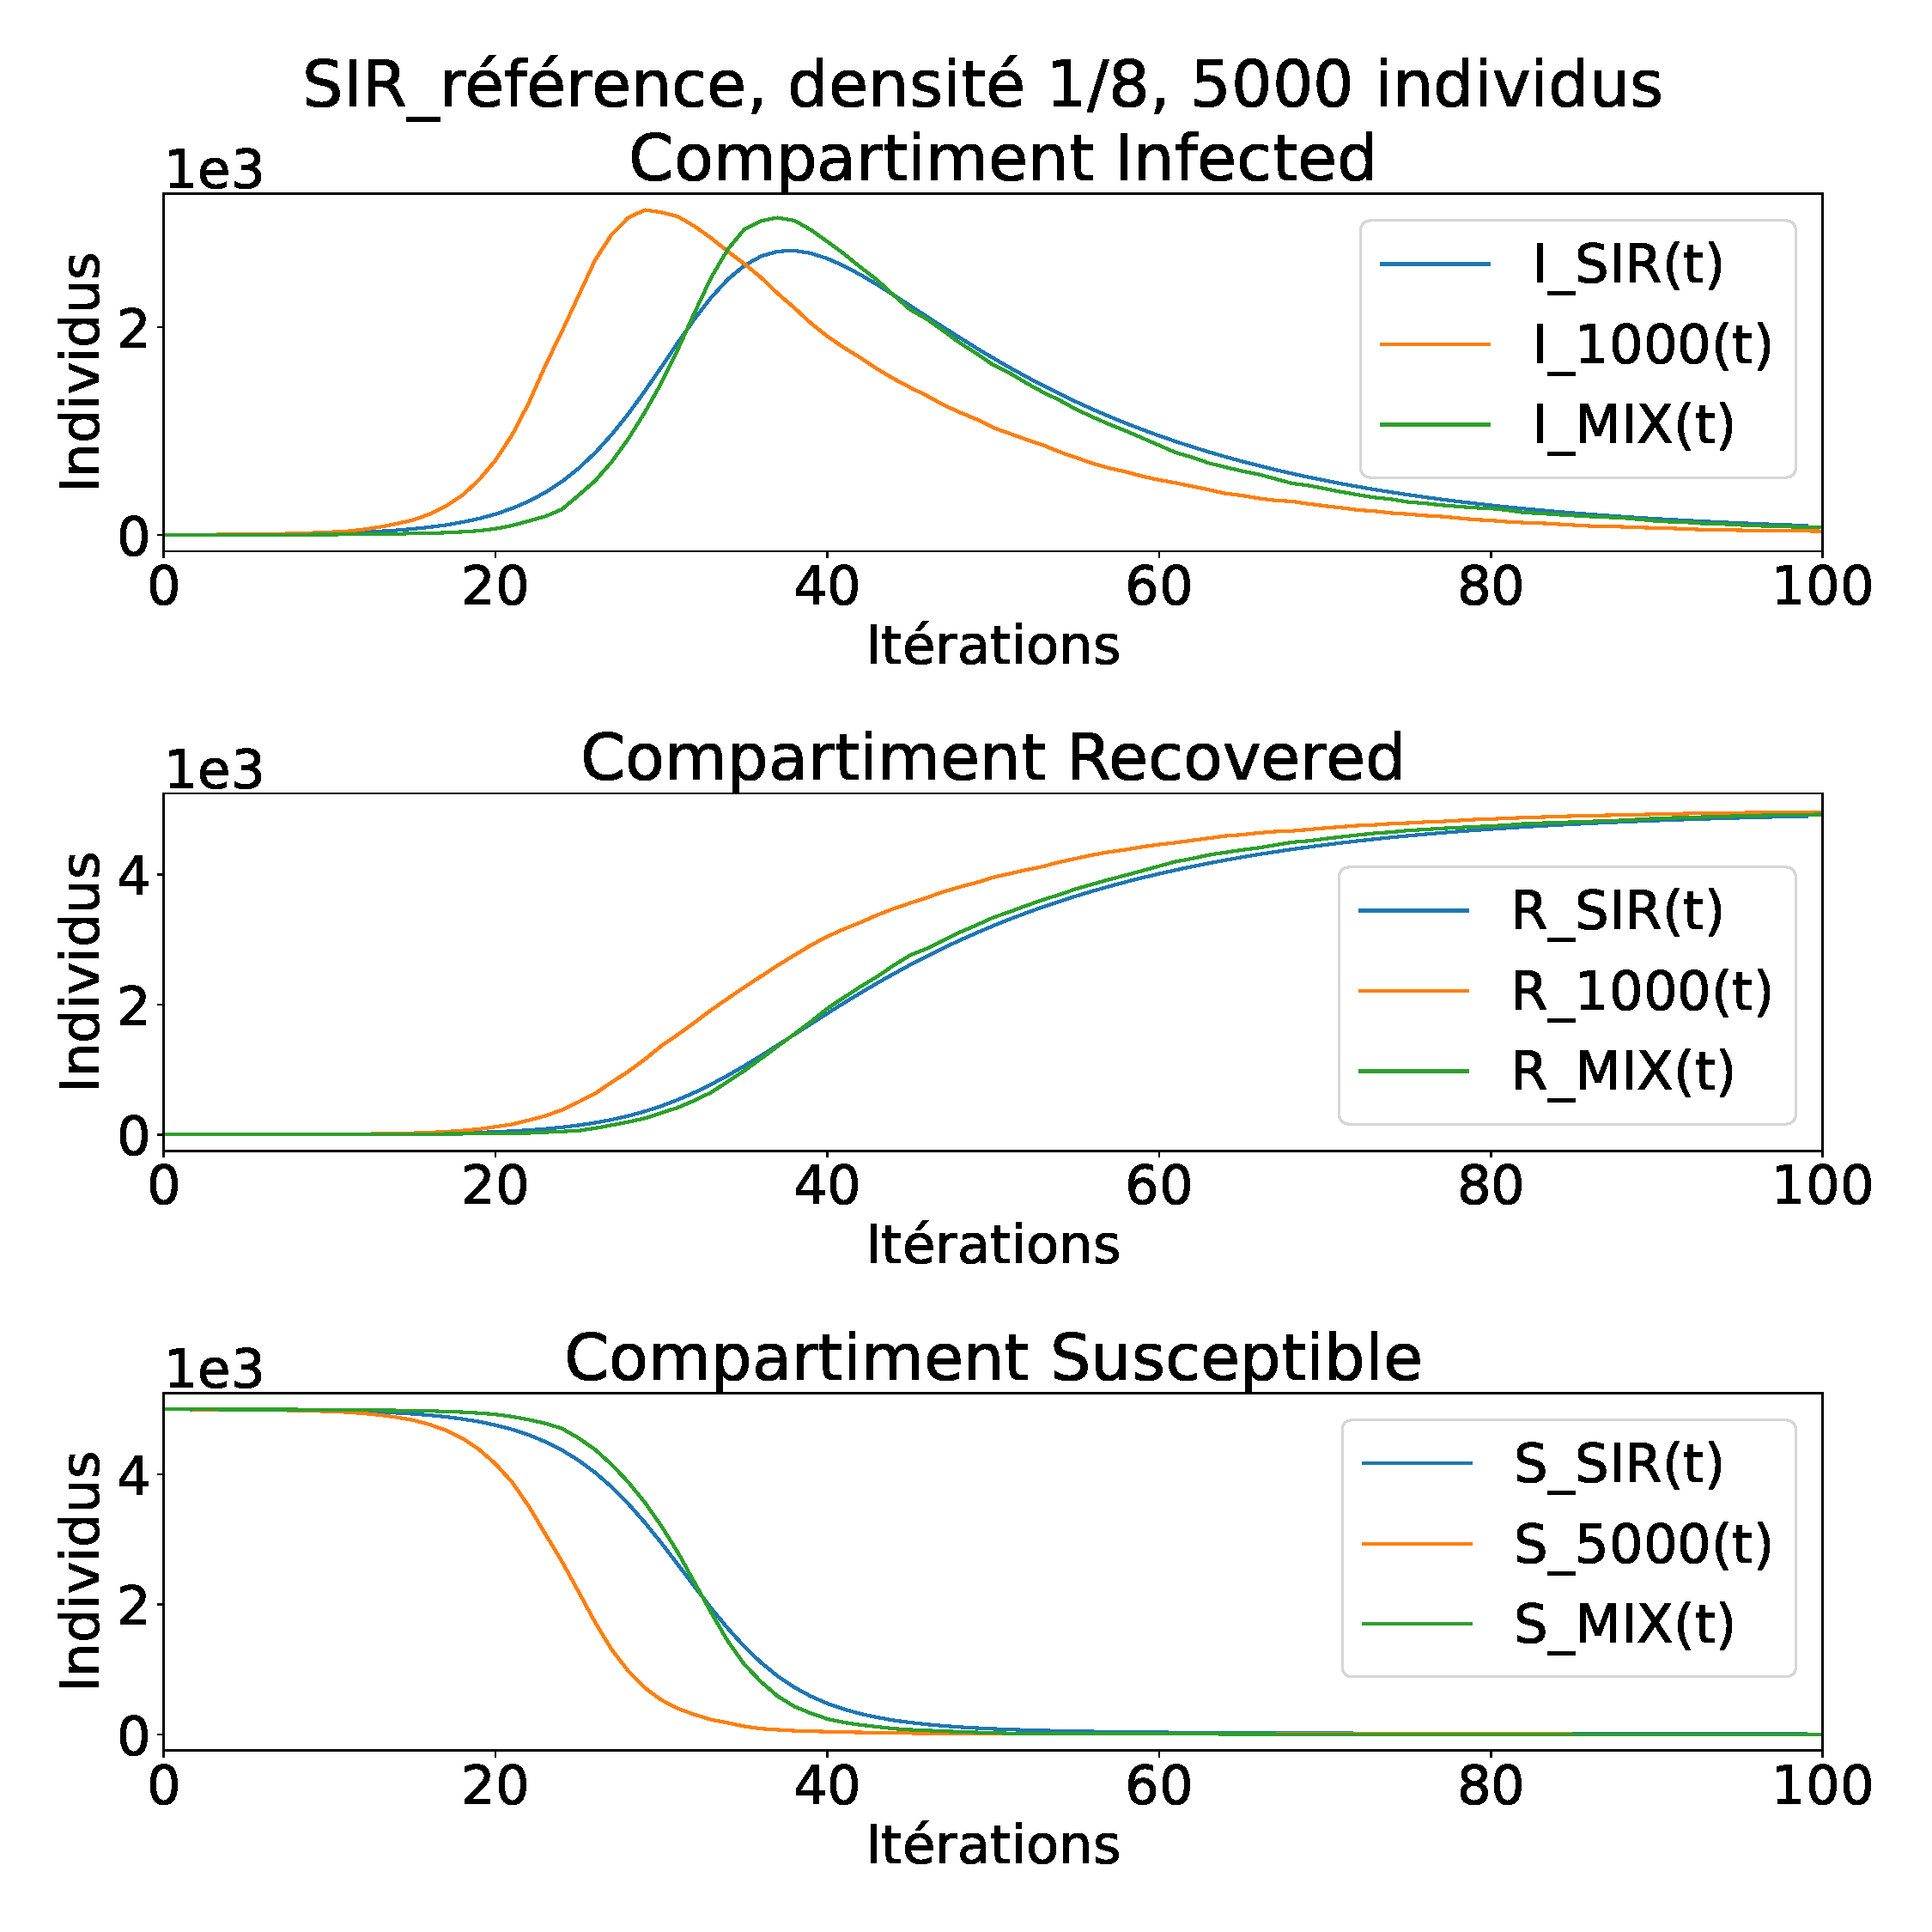
\includegraphics[width=.6\textwidth]{Images/SIR_ref_8_5.pdf}
	\caption[Simulation SIR avec latence]{Exemple de simulation SIR avec de la latence. La courbe bleue représente le modèle mathématique, la verte la simulations au mélange parfait et la orange la simulations aux $1000$ mouvements. Nous nous intéressons ici au mauvais fit du modèle mathématique sur la courbe de la simulation au mélange parfait.}
\end{figure}

Pour confirmer la théorie de la latence, nous ajoutons une latence artificielle au modèle SIR et regardons l'impacte sur le "mean absolute error". En effet, si la simulation a quelques itérations de latence, nous devrions pouvoir ajouter de la latence au modèle SIR et observer des améliorations sur le MAE.

\newpage

\begin{figure}[h]
    \centering
	\captionsetup{justification=centering}
	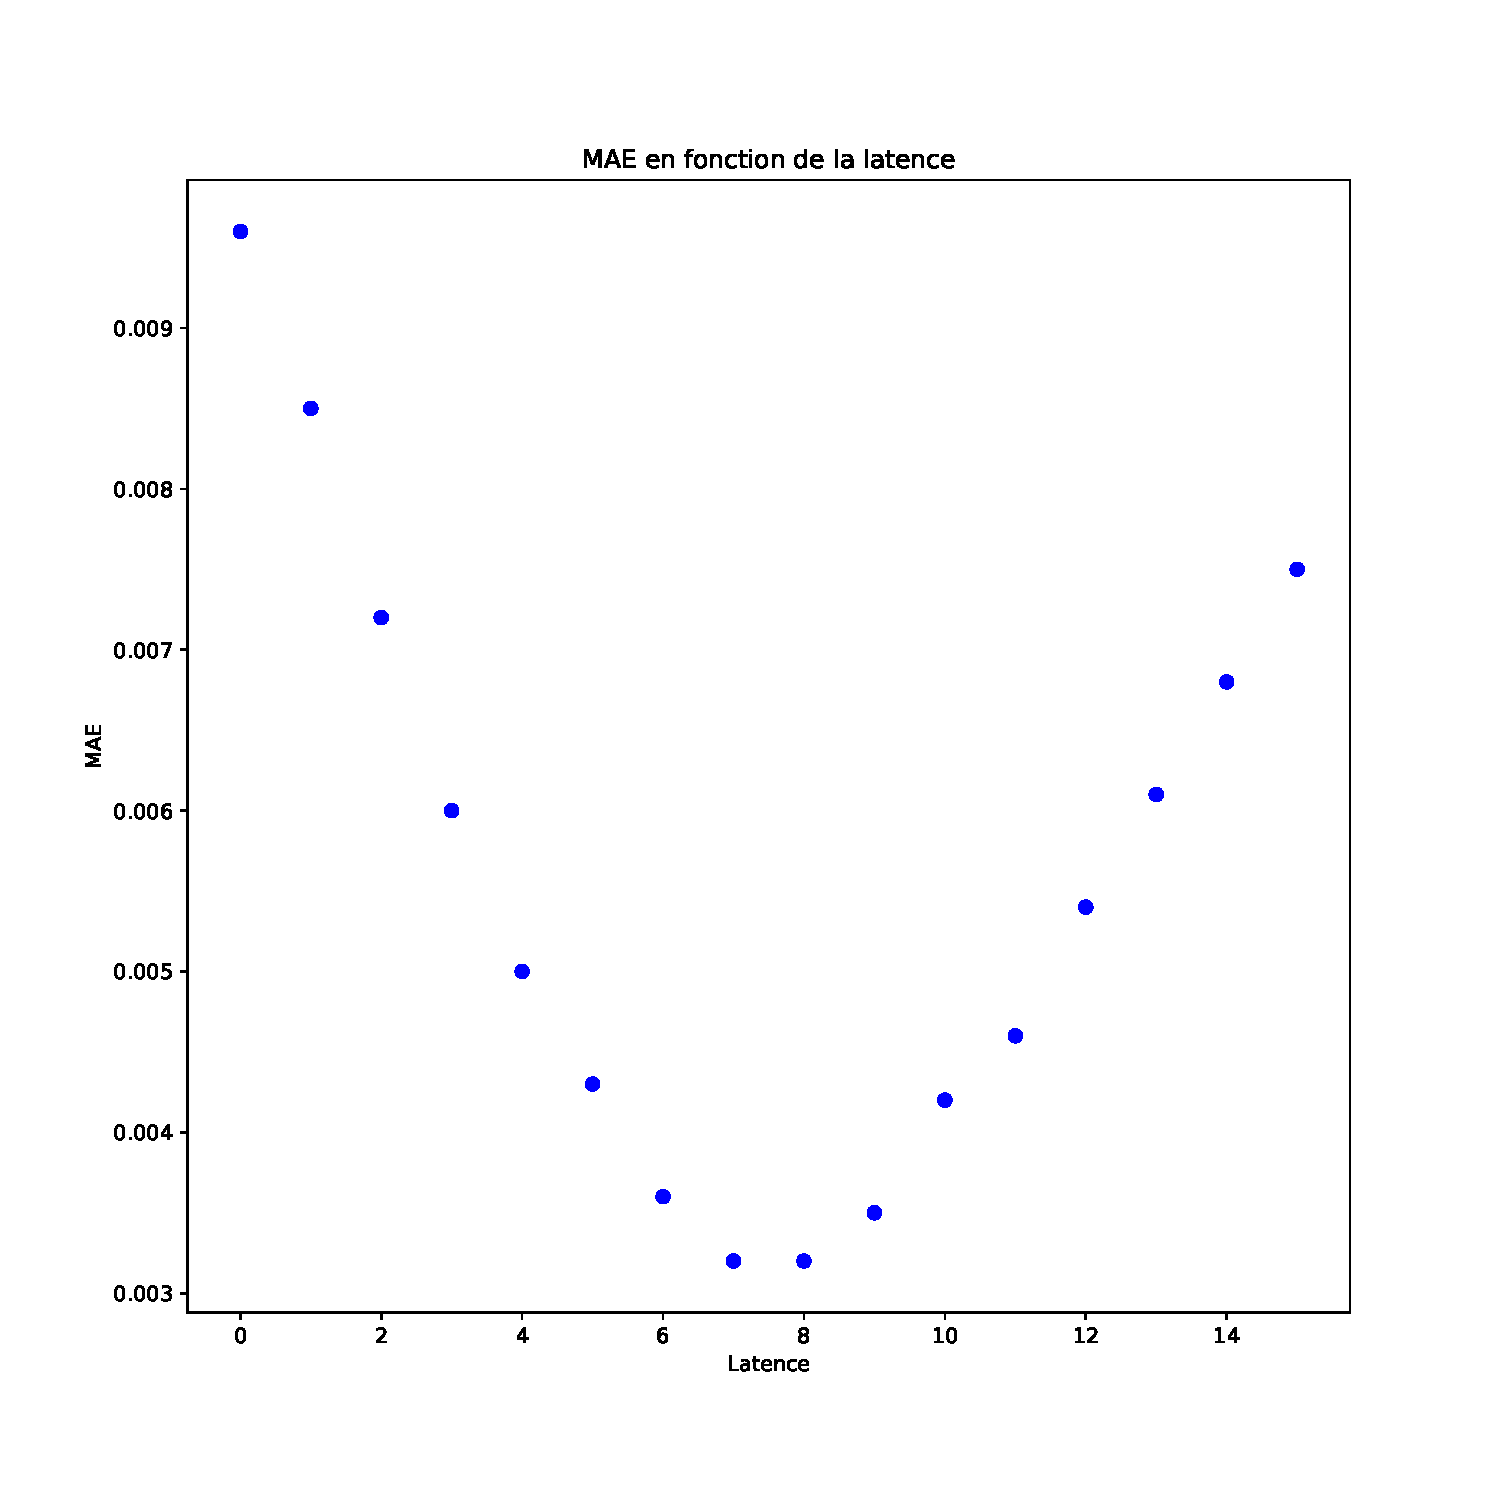
\includegraphics[width=.7\textwidth]{Images/SIR_latence_8_5.pdf}
	\caption[Mesures de latences SIR]{Mesure de la latence de la simulation au mélange parfait. Sur les abscisses nous avons la latence artificielle que nous ajoutons au modèle SIR et sur les ordonnées nous avons le MAE entre le modèle mathématique et la simulation. L'idée est d'ajouter de la latence au modèle mathématique afin de chercher un meilleur fit.}
\end{figure}

La figure ci-dessus montre la valeur du MAE en ajoutant de la latence au modèle SIR. Sur les abscisses nous avons le nombre d'itérations de latence ajoutée à SIR et sur l'axe des ordonnées nous avons le calcul du MAE entre le modèle mathématique et la simulation au mélange parfait.\\

La valeur minimale de MAE est atteinte avec une latence artificielle sur SIR de $7$ itérations. Ce qui veut dire que notre simulation subit une latence de $7$ itéraitons.

\newpage

\subsection{Mouvements variable}

Jusqu'à présent, toutes les simulations ont utilisé une des deux méthodes de déplacement : mélange parfait ou $1000$ mouvements. Nous sommes partis de l'hypothèse que plus le nombre de mouvements est grand, plus le modèle tend vers la méthode du mélange parfait.\\

Ce paragraphe est destiné à visualiser l'impacte du nombre de mouvements sur le déroulement d'une simulation. La même simulation est exécutée une fois avec le mode de mélange parfait et $9$ fois avec un nombre de mouvements variable : $1$, $10$, $50$ ,$100$, $200$, $400$, $600$, $800$, $1000$ mouvements.

\begin{figure}[h]
	\centering
	\captionsetup{justification=centering}
	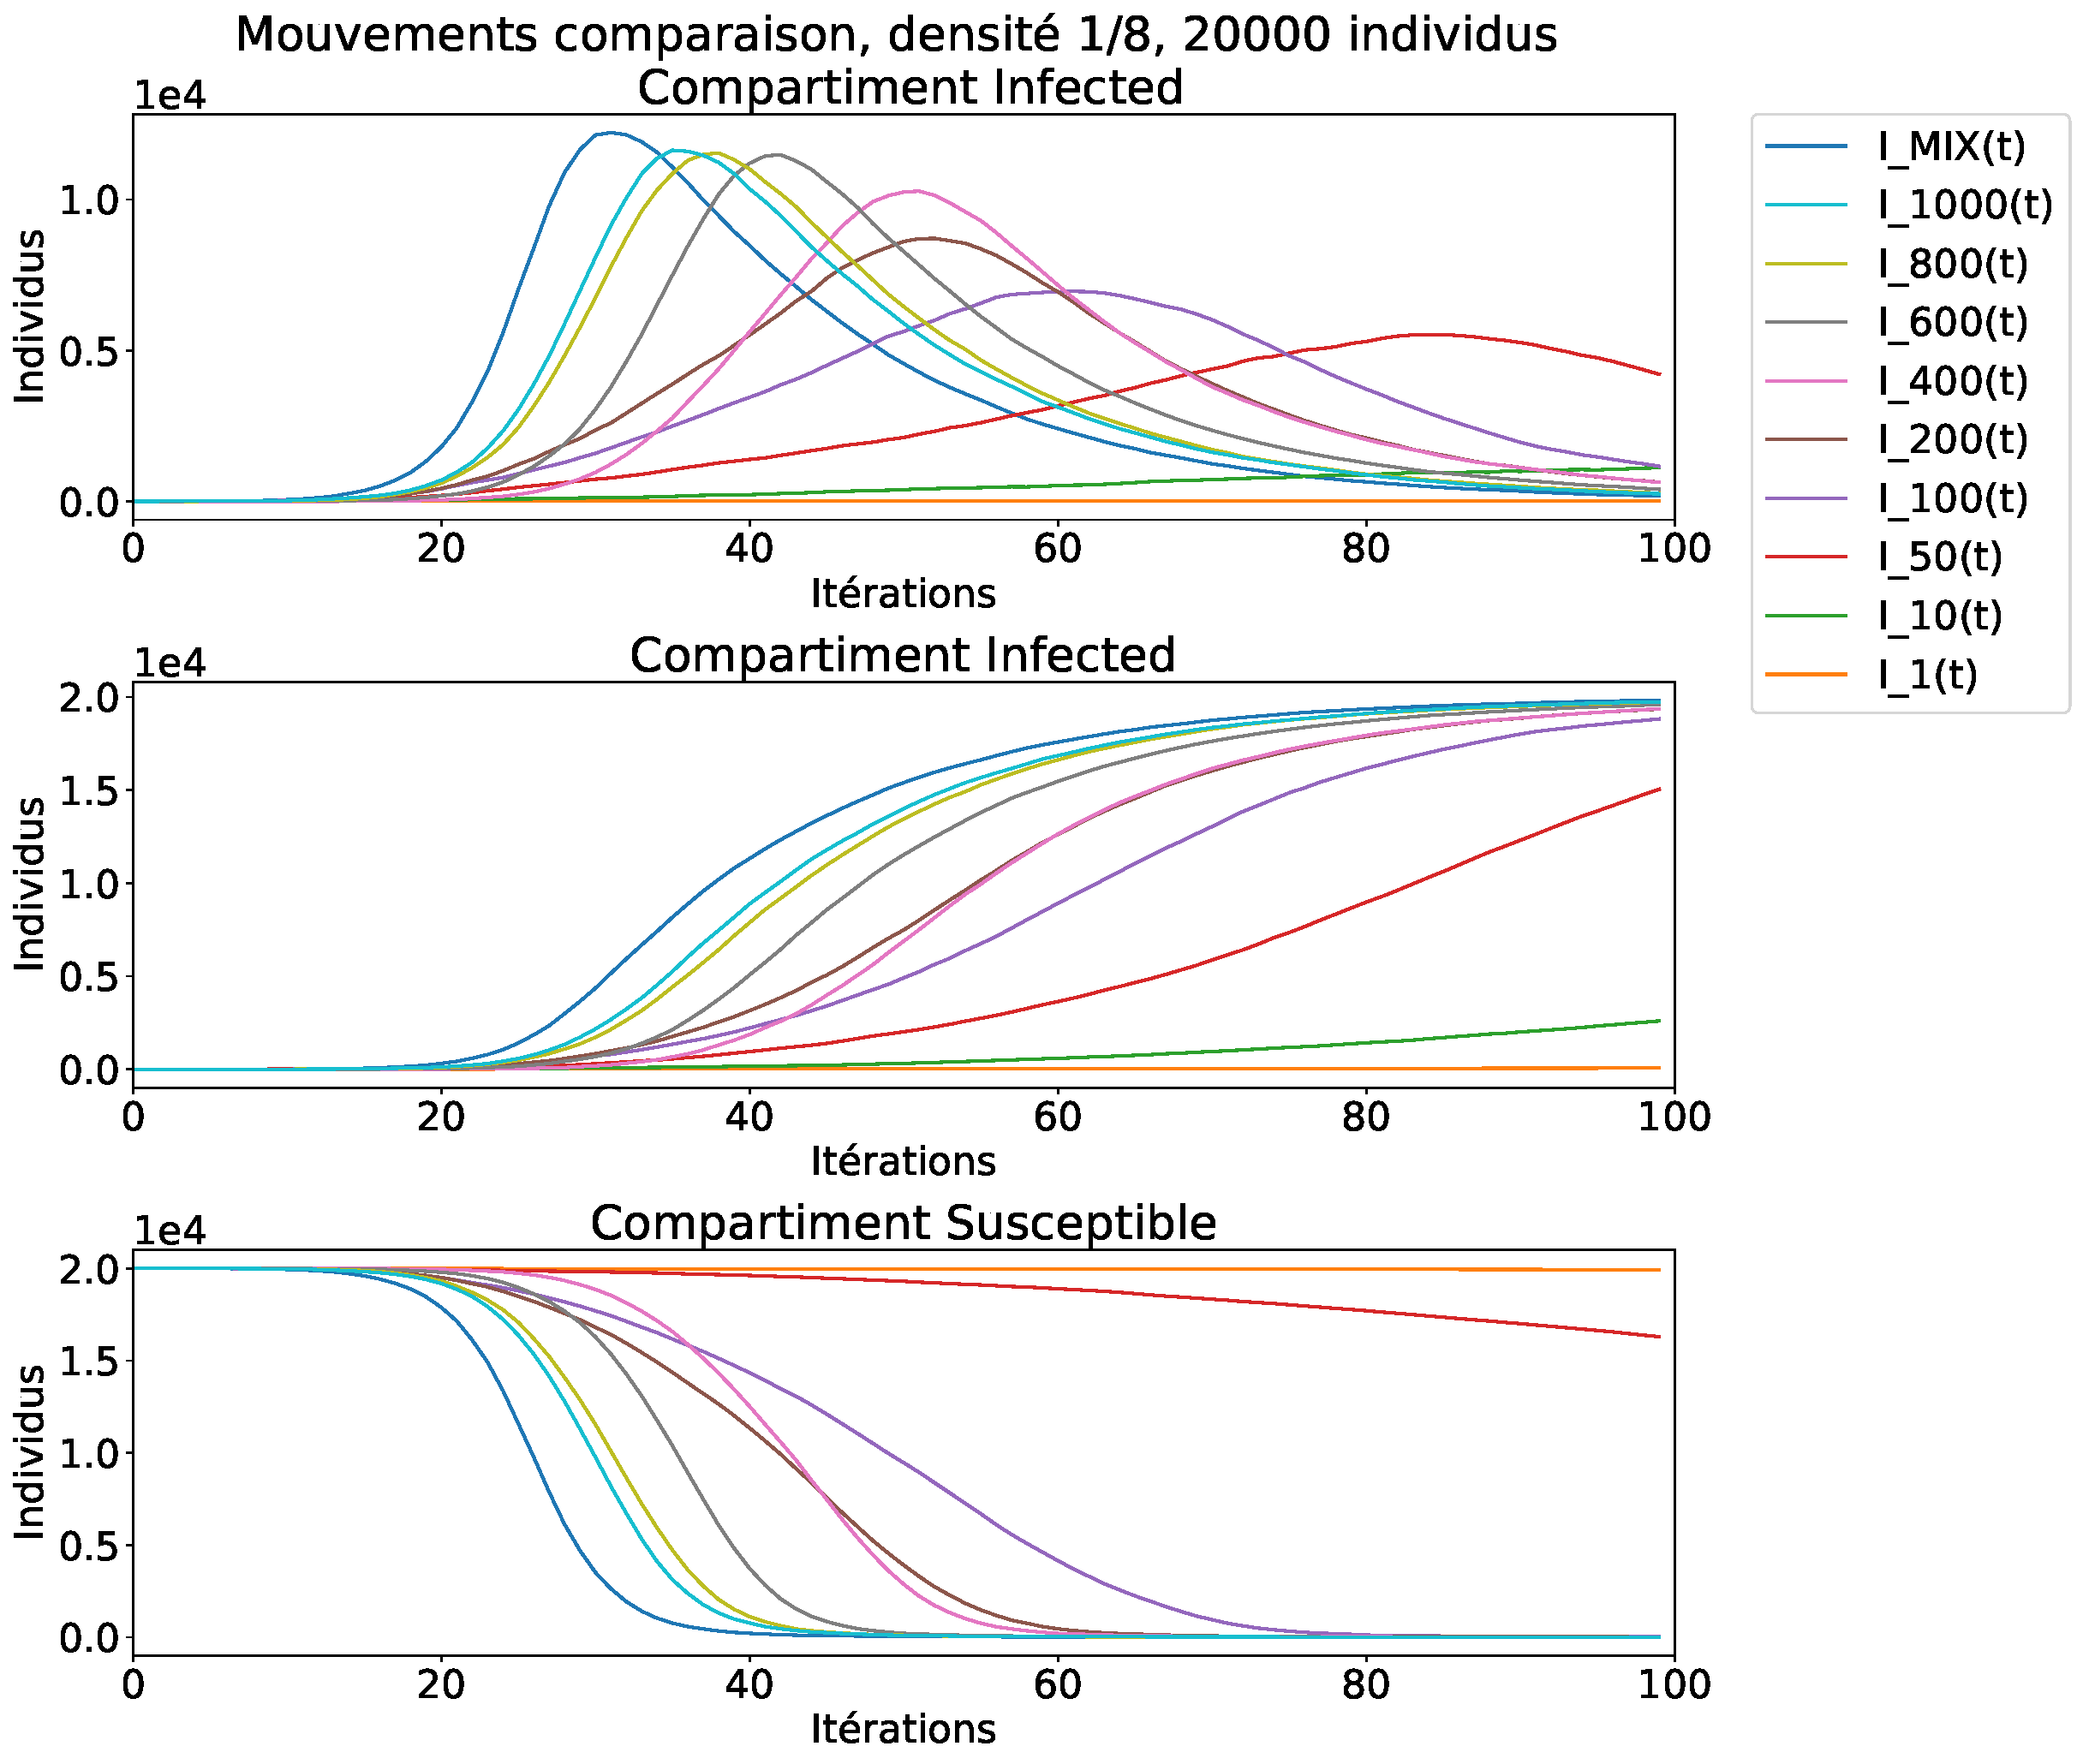
\includegraphics[width=.8\textwidth]{Images/SIR_mouvements_variables.pdf}
	\caption[Mouvements variable : SIR]{Comparaison de simulations aux mêmes paramètres avec des nombres de mouvements par individu variant. Les simulations vont de un seul mouvements par itération et par individu à $1000$ mouvements. La courbe au mélange parfait est aussi présente comme référence.}
\end{figure}

Les résultats suivent notre intuition. Plus le mélange est efficace, plus la pandémie est rapide. Par conséquent, le nombre de mouvements a un impact direct sur la propagation de pandémies et ceci significativement. 

\newpage

\subsection{Comparaison 1000 mouvements}

Afin d'étudier la scalabilité du modèle sur de grandes simulations, nous comparons des simulations aux mêmes paramètres et même densité mais de taille différente. Le but est d'observer les différences entre des simulations presque identiques mais de taille différente. Pour pouvoir comparer des simulations de population différente il faut normaliser les résultats, c'est-à-dire diviser les valeurs par le nombre d'individus.\\

Les figures qui suivent superposent les $4$ simulations faites pour une densité en les normalisant par la taille de la population. Pour chaque densité étudiée, les simulations ont été réalisée avec des populations de $5000$, $20000$, $50000$ et $100000$ individus. Sur les figures, les courbes bleues appartiennent aux simulations à $5000$ individus, les courbes oranges aux simulations à $20000$ individus, les bleues aux simulations à $50000$ individus et finalement les rouges aux simulations à $100000$ individus. Les figures de gauche superposent les simulations de densité $1/2$ et celles de droite montrent les simulations de denstié $1/16$.

\begin{figure}[h]
	\centering
	\captionsetup{justification=centering}
	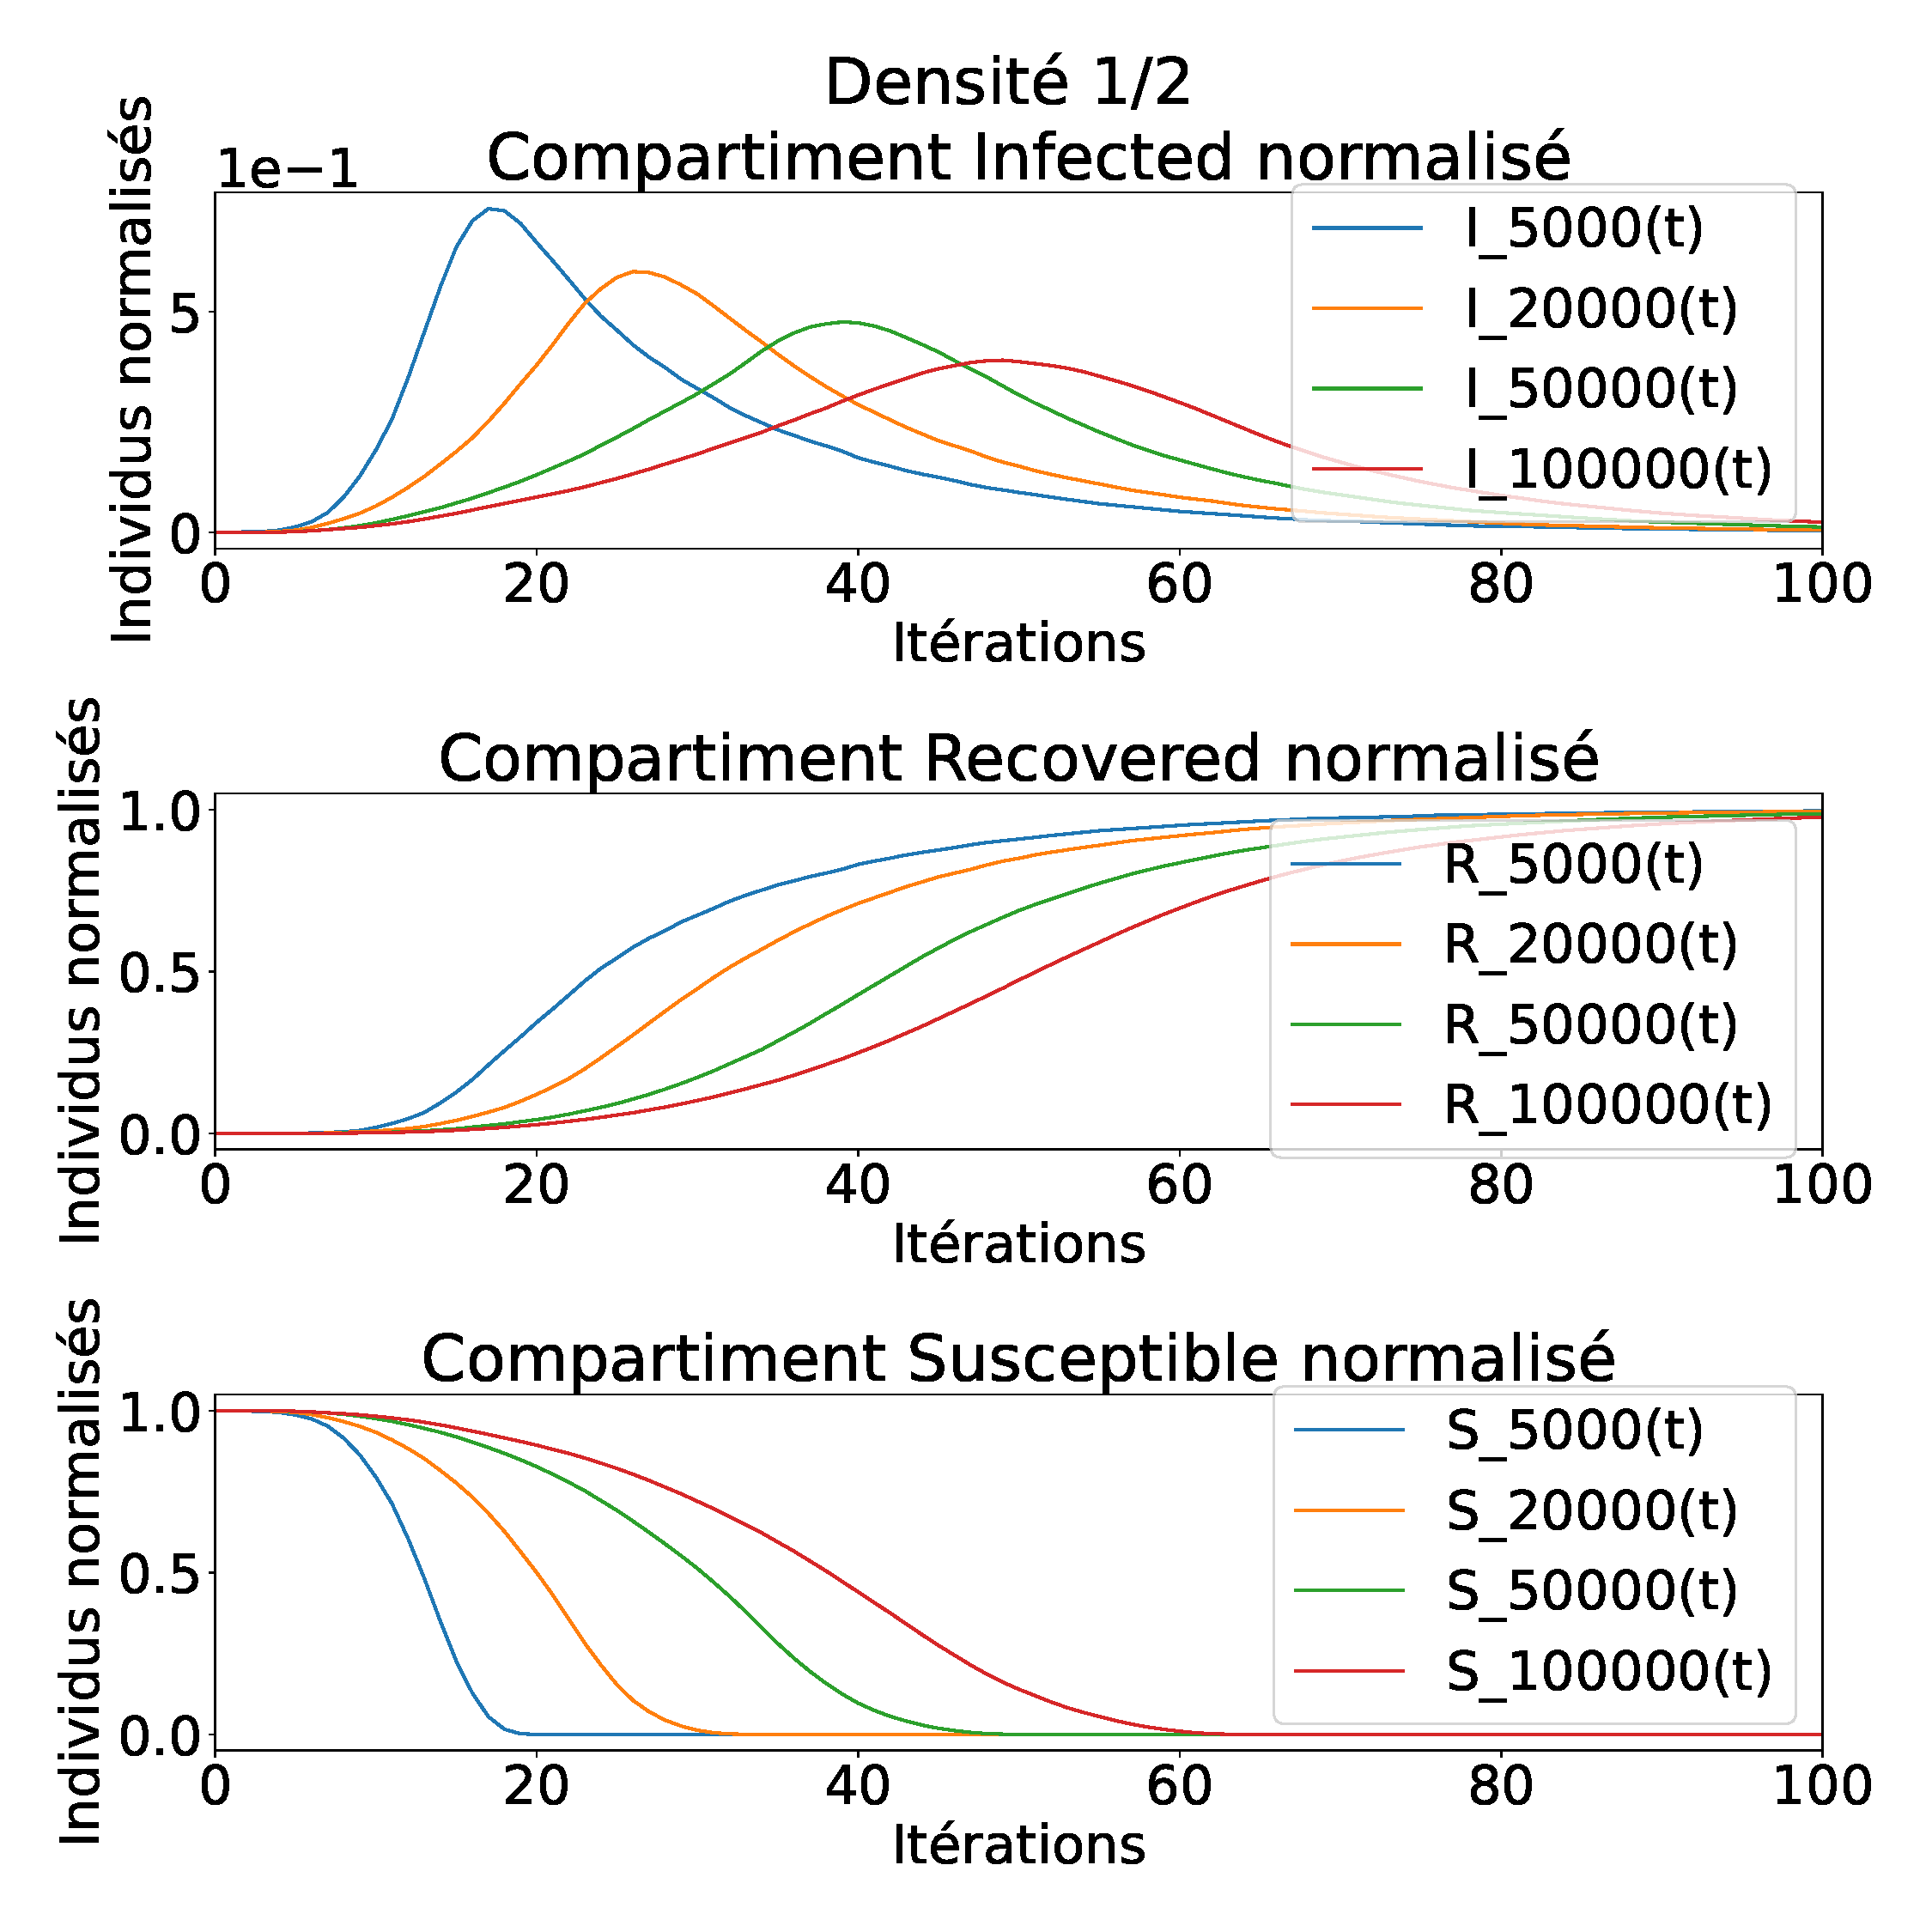
\includegraphics[width=.49\textwidth]{Images/SIR_1000_2.pdf}
	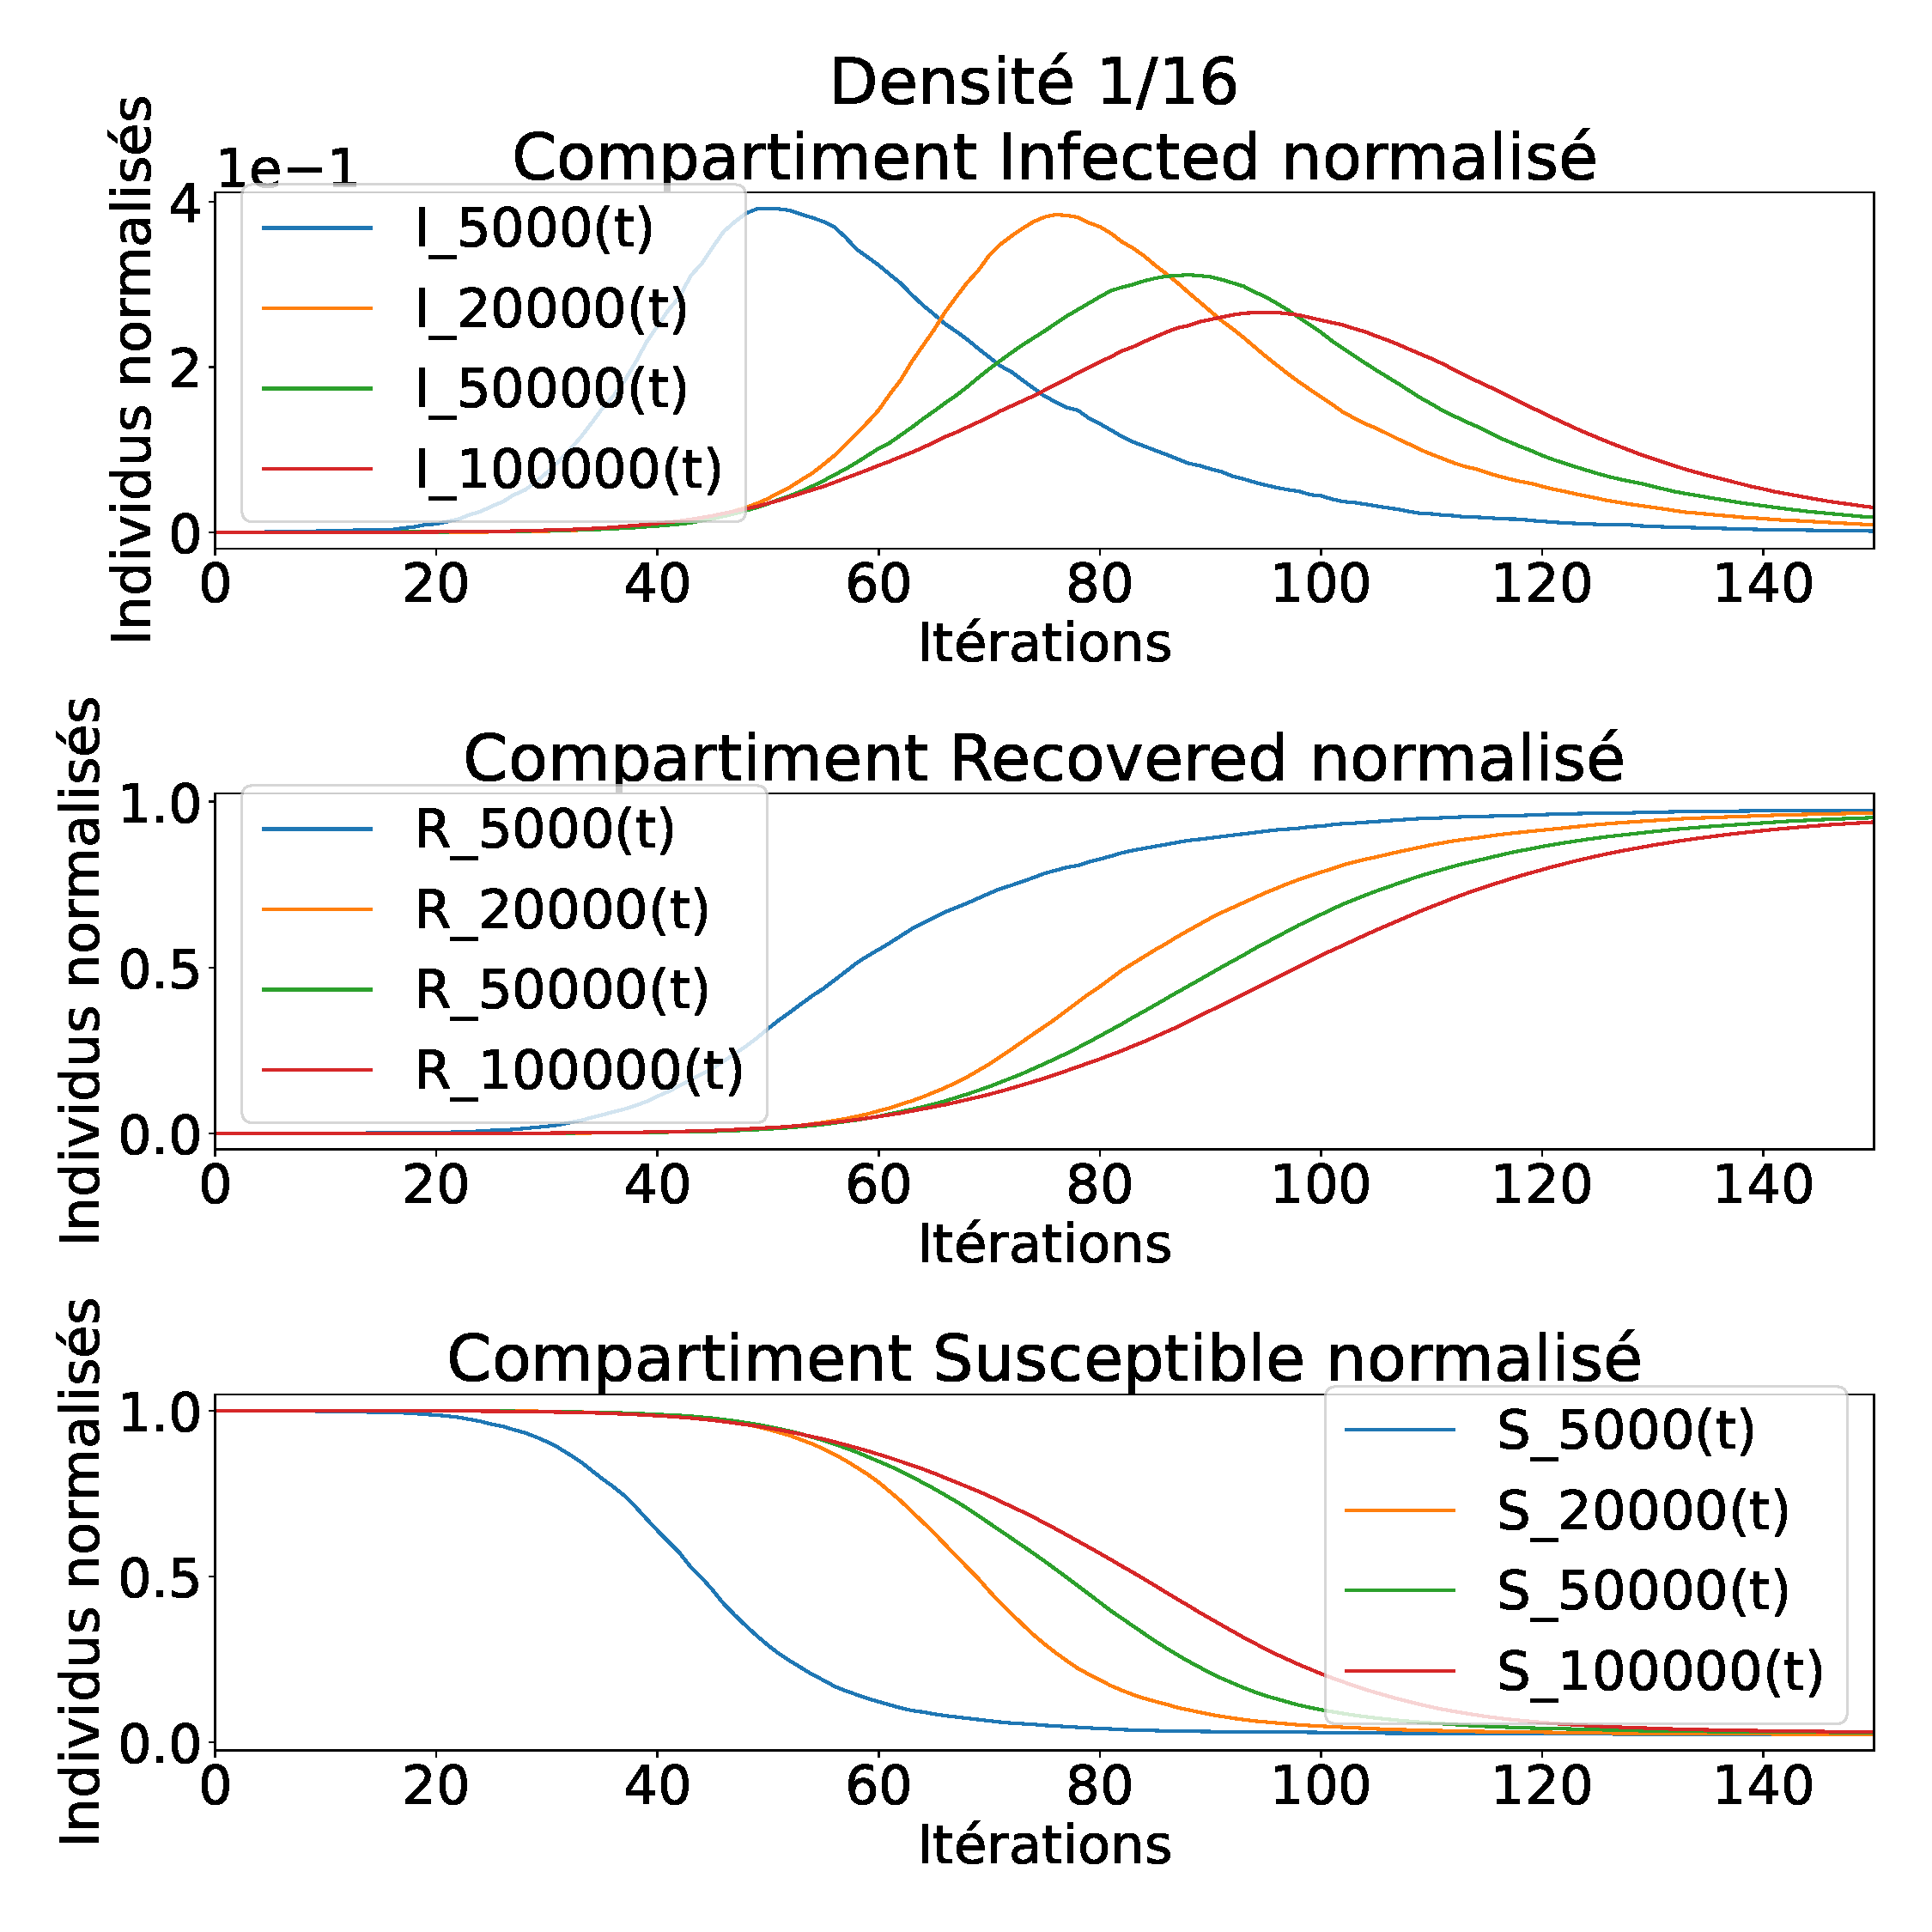
\includegraphics[width=.49\textwidth]{Images/SIR_1000_16.pdf}
	\caption[Comparaison simulations SIR normalisées]{Comparaison des simulations SIR normalisées par le nombre d'individus. Superposition des $4$ simulations aux tailles de population différentes en densité $1/2$ à gauche et en densité $1/16$ à droite. Les courbes bleues appartiennent aux simulations à $5000$ individus, les courbes oranges aux simulations à $20000$ individus, les bleues aux simulations à $50000$ individus et finalement les rouges aux simulations à $100000$ individus. Les figures de gauche superposent les simulations de densité $1/2$ et celles de droite montrent les simulations de denstié $1/16$}
\end{figure}

Nous pouvons observer deux phénomènes. Le premier est le fait que plus le nombre d'individus est élevé, plus la pandémie prend du temps à se propager, ce qui paraît assez logique car il faut contaminer d'avantage d'individus. Le deuxième phénomène est le fait que le pic d'infectés décroît lorsque nous augmentons le nombre d'individus. Mais cette décroissance n'est pas constante sur les quatre densités testées. En effet il semblerait que plus la densité soit élevée, plus les variations entre les pics sont grands.\\

Ce dernier phénomène est conforme à ce que nous avons étudié précédemment. Les systèmes à forte densité peinent à se mouvoir et propager une pandémie. Par conséquent le rayon de propagation de la pandémie est fixe pour une certaine densité et ne dépend pas du nombre d'individus. Nous avons donc les systèmes à forte densité et grande taille qui peinent à contaminer la population, ce qui produit des événement plus progressif et donc avec un pic de contaminés moins élevé. Par contre les simulations moins denses pénalisent moins les grands systèmes car le mélange s'effectue mieux. Avec un bon mélange, le nombre de personnes n'impacte pas la vitesse de propagation. Cette situation est comparable à concaténer plusieurs simulations de plus petite taille pour en obtenir une grande. Dans cette configuration, les $N$ simulations constituant la grande ne prennent pas $N$ fois plus de temps que l'exécution d'une seule.
